%% Latex template for PhD dissertation or MS thesis
%% Department of Mechanical Engineering
%% Brigham Young University
%% Last Modified: June 2016

\documentclass[12pt,twoside]{report}% Use this line for the print version of the thesis
%\documentclass[12pt,oneside]{report}% If you comment out the line above, and uncomment this line, it will create a file without the extra pages that the Library wants for its electronic file versions.

%%%%%%%%%%%%%%%%%%%%%%%%%%%%%%%%%%%%%%%%%%%%%%%%%%%%%%%%%
%  Setup BYU thesis format
%%%%%%%%%%%%%%%%%%%%%%%%%%%%%%%%%%%%%%%%%%%%%%%%%%%%%%%%%
\usepackage{byustyle}
% Setup the byu style sheet
\byustylesetup{%
    %
    %isdissertation = true,            % Uncomment this if you're doing a PhD dissertation
    %
    % Definitions of names needed in thesis/dissertation
    deptname          = {Department of Electrical and Computer Engineering},    %
    committeechairman = Michael Rice,                      %
    committeemembera  = Brian D. Jeffs,                         %
    committeememberb  = Karl F. Warnick,                          %
    %graddate = April 2011,  		% Final approval month (NOT graduation month!        	
     %
    %Uncomment to shorten for proofreading purposes
    %noabstract = true,         % Don't show the abstract page
    %nouniversitypages = true,  % Don't show any of the "university pages"
    %noacknowledgements = true, % Don't show the Acknowledgements page
    %notableofcontents = true,  % Don't show the Table of Contents
    %nolistoffigures = true,    % Don't show the List of Figures
    %nolistoftables = true,     % Don't show the List of Tables
    %nolistoflistings = true,
    nonomenclature = true,     % Don't show the Nomenclature section - note that this section is optional
    %notocandlists = true,      % Don't show the Table of Contents, List of Figures, or the List of Tables
    %noheaderatall = true,      % Don't show any of the BYU Thesis header pages
    keywords = {equalization, SOQPSK-TG, GPU, CUDA, aeronautical telemetry} % Enter your keywords
%inside the curly braces, as you'd like them to appear on the bottom of the abstract page.
}
%%%%%%%%%%%%%%%%%%%%%%%%%%%%%%%%%%%%%%%%%%%%%%%%%%%%%%%%
%  Include other \usepackage{} statements here.
%    Add one package at a time.
%    Warning:  Some packages are not compatible with byuthesis.sty
%%%%%%%%%%%%%%%%%%%%%%%%%%%%%%%%%%%%%%%%%%%%%%%%%%%%%%%%%
% You should turn on any of these that you think you'll need!

%\usepackage[normalmargins]{savetrees} 	% prints smaller to save trees (draft only)
\usepackage{amsmath}										%	allows for mathematical symbols
\usepackage{mathrsfs,amsmath}
\usepackage{amssymb}										%	defines symbol names for all the math symbols
\usepackage{graphicx}        						% for .pdf graphics inclusion
%\usepackage{subfigure}									%	allows for subfigures
\usepackage{caption}
\usepackage[calcwidth = 6in]{caption}
\usepackage{booktabs,threeparttable}
\usepackage{dcolumn}
\usepackage{subcaption}	
\usepackage{setspace}										%	change the spacing inside a document
\usepackage{epstopdf}										%	converts a .eps to a .pdf
\usepackage{cite}												%	allows for citations
\usepackage{mathptmx}
\usepackage{textcomp}
\usepackage{float}											%	improves the interface for defining floating objects
\usepackage{rotating}
\usepackage{listings}
\usepackage{xcolor}
\usepackage{nicefrac}
%\usepackage[figuresright]{rotfloat}
%\usepackage{multirow}
%These next two lines are for the citing with the IEEE style (leave commented for ASME)
%\renewcommand\citepunct{], [}
%\renewcommand\citedash{]--[}
%%%%%%%%%%%%%%%%%%%%%%%%%%%%%%%%%%%%%%%%%%%%%%%%%%%%%%%%
% For doing bookmarks in the PDF file
%%%%%%%%%%%%%%%%%%%%%%%%%%%%%%%%%%%%%%%%%%%%%%%%%%%%%%%%%
% For more info, see:
% http://www.geocities.com/kijoo2000/latex2pdf.pdf
% http://www.tug.org/applications/hyperref/manual.html
\usepackage[pdftex,backref,pagebackref,plainpages=false]{hyperref}
\hypersetup{
    %bookmarks    = true, % Make bookmarks (default=true). This option
                          %cannot be used after package has been loaded,
                          %thus use like this: \usepackage[bookmarks=false]{hyperref}.
    %
    breaklinks   = false, % Allow link text to break across lines (default=false).
    linktocpage  = false, % make page number, not text, be link on TOC, LOF and LOT
    colorlinks   = false, % Color the text of links (true) or put color frames over
    %
    linkbordercolor  = {1 1 1}, % The color of the box around normal links (white so they won't show up)
    citebordercolor  = {1 1 1}, % The color of the box around citations (white so they won't show up)
                          % the links (false).
    pdfstartview = {FitV}, % Set the startup page view. Possible options are:
                           % FitH: Fit whole width of page
                           % FitV: Fit whole height of page
                           % FitB: Fit whole �Bounding Box� page
                           % FitBH: Fit whole width of �Bounding Box� of page
                           % FitBV: Fit whole height of �Bounding Box� of page
    bookmarksnumbered  = true, % Put section numbers in bookmarks (default=false)
    bookmarksopen      = true, % Open up the bookmark trees (default=false).
    bookmarksopenlevel = 0, % Level to which bookmarks are open (default=\maxdimen).
    bookmarkstype      = toc, % Specify which toc file to mimic (default=toc).
    pdfpagemode        = {UseOutlines}, %  Specify how document starts when opened ({None}).
                                        % Possible options are:,
                                        % None: Neither bookmarks nor thumbnails are visible.
                                        % UseOutlines: Bookmarks are visible.
                                        % UseThumbs: Thumbnails are visible.
                                        % FullScreen: Full-screen mode
    pdftitle    = {GPU Implementation of Data-Aided Equalizers},
    pdftitle    = {GPU Implementation of Data-Aided Equalizers},
    pdfauthor   = {Jeffrey Thomas Ravert},
    pdfcreator  = {Jeffrey Thomas Ravert},
    pdfsubject  = {Jeffrey Thomas Ravert's Master's Thesis},
    pdfkeywords = {equalization, SOQPSK-TG, GPU, CUDA, aeronautical telemetry},
    pdfborder		=	{0 0 0},}
%%%%%%%%%%%%%%%%%%%%%%%%%%%%%%%%%%%%%%%%%%%%%%%%%%%%%%%%
%  Define macros here - You may use these, or delete them, as you see fit.
%%%%%%%%%%%%%%%%%%%%%%%%%%%%%%%%%%%%%%%%%%%%%%%%%%%%%%%%%
\lstdefinestyle{myCUDAstyle} {
	language=[ANSI]C++,
    showstringspaces=false,
    backgroundcolor=\color{mygray},
    basicstyle=\lstfont{black},
    identifierstyle=\lstfont{black},
    keywordstyle=\lstfont{magenta},
    numberstyle=\lstfont{black},
    stringstyle=\lstfont{cyan},
    commentstyle=\lstfont{yellow!30!black},
    moredelim=[is][\lstfont{green!50!black}]{@}{@},
    emph={
        cudaMalloc, cudaFree,
        cudaMallocHost, cudaFreeHost,
        cudaMemcpyAsync, cudaMemcpy, cudaMemcpyHostToDevice, cudaMemcpyDeviceToHost,
        cudaSuccess, cudaGetLastError, cudaGetErrorString,
        cudaErrorMemoryAllocation, cudaError_t,
        cudaOccupancyMaxPotentialBlockSize,
        __global__, __shared__, __device__, __host__,
        __syncthreads,
        cudaEvent_t, cudaStream_t,
        cudaEventCreate, cudaEventSynchronize, cudaEventDestroy,
        cudaEventElapsedTime, cudaEventQuery, cudaEventRecord,
        cudaStreamWaitEvent,
        threadIdx, blockIdx, blockDim, gridDim,
        cudaStream_t, cudaStreamCreate, cudaStreamDestroy,
        cudaMemcpyDeviceToDevice, cudaMemcpyHostToHost,
    },
    emphstyle={\lstfont{green!50!black}},
    breaklines=true,
    numbers=left
    }
    
    \lstdefinestyle{myCUDAstyle_inline} {
	language=[ANSI]C++,
    showstringspaces=false,
    backgroundcolor=\color{white},
    basicstyle=\lstfont{black},
    identifierstyle=\lstfont{black},
    keywordstyle=\lstfont{magenta},
    stringstyle=\lstfont{cyan},
    commentstyle=\lstfont{yellow!30!black},
    moredelim=[is][\lstfont{green!50!black}]{@}{@},
    emph={
        cudaMalloc, cudaFree,
        cudaMallocHost, cudaFreeHost,
        cudaMemcpyAsync, cudaMemcpy, cudaMemcpyHostToDevice, cudaMemcpyDeviceToHost,
        cudaSuccess, cudaGetLastError, cudaGetErrorString,
        cudaErrorMemoryAllocation, cudaError_t,
        cudaOccupancyMaxPotentialBlockSize,
        __global__, __shared__, __device__, __host__,
        __syncthreads,
        cudaEvent_t, cudaStream_t,
        cudaEventCreate, cudaEventSynchronize, cudaEventDestroy,
        cudaEventElapsedTime, cudaEventQuery, cudaEventRecord,
        cudaStreamWaitEvent,
        threadIdx, blockIdx, blockDim, gridDim,
        cudaStream_t, cudaStreamCreate, cudaStreamDestroy,
        cudaMemcpyDeviceToDevice, cudaMemcpyHostToHost,
    },
    emphstyle={\lstfont{green!50!black}},
    breaklines=true,
    }

\definecolor{codenumber}{rgb}{0.5,0.5,0.5}
\definecolor{codekeyword}{rgb}{0.9,0.4,0.7}
\definecolor{codeCUDA}{rgb}{1.0,0.6,0.6}
\newcommand{\lst}[1]{\colorbox{white!20!black}{\lstinline!#1!}}
\newcommand{\lstfont}[1]{\color{#1}\scriptsize\ttfamily}
\newcommand{\lsttinyfont}[1]{\color{#1}\fontsize{7}{7}\ttfamily}
\newcommand{\lstinlinefont}[1]{\color{#1}\scriptsize\ttfamily}
\definecolor{mygray}{rgb}{0.97,0.97,0.97}

\def\proof{\noindent{\it Proof: }}
\def\QED{\mbox{\rule[0pt]{1.5ex}{1.5ex}}}
\def\endproof{\hspace*{\fill}~\QED\par\endtrivlist\unskip}
\newcommand{\norm}[1]{\left\|#1\right\|}
\newcommand{\abs}[1]{\left|#1\right|}
\newcommand{\defeq}{\stackrel{\triangle}{=}}
\newcommand{\re}{\mathbb{R}}																			% real numbers
\newcommand{\OMIT}[1]{{}} 																			% omit sections of text
\newcommand{\pd}[2]{\ensuremath{\frac{\partial #1}{\partial #2}}} % partial derivative
\newcommand{\superscript}[1]{\ensuremath{^\textrm{#1}}}
\newcommand{\subscript}[1]{\ensuremath{_\textrm{#1}}}
\newcommand{\rpkt}{\mathbf{r}_\text{pkt}}
\newcommand{\Lpkt}{L_\text{pkt}}
\newcommand{\Lp}{L_\text{p}}
\newcommand{\Lasm}{L_\text{ASM}}
\newcommand{\Ldata}{L_\text{d}}

\DeclareCaptionJustification{InvertedPyramid}{\hsize=6in
                \parindent=0pt
                \leftskip=0pt plus.5fil
                \rightskip=0pt plus-0.5fil
                \parfillskip=0pt plus1fil
                \emergencystretch=1in
                \parshape10
                0.00in \linewidth
                0.025\linewidth 0.95\linewidth
                0.05\linewidth 0.9\linewidth
                0.075\linewidth 0.85\linewidth
                0.1\linewidth 0.8\linewidth
                0.125\linewidth 0.75\linewidth
	     0.15\linewidth 0.70\linewidth
	     0.175\linewidth 0.65\linewidth
	     0.2\linewidth 0.60\linewidth
	     0.225\linewidth 0.55\linewidth
                \strut
	} 
\renewcommand{\TPTminimum}{3in}
\captionsetup[table]{justification=InvertedPyramid} 
\captionsetup[lstlisting]{justification=InvertedPyramid} 

\newsavebox{\tempbox}
\newlength{\tempwidth}

%%%%%%%%%%%%%%%%%%%%%%%%%%%%%%%%%%%%%%%%%%%%%%%%%%%%%%%%
% To only print a few chapters without changing the reference numbers, 
%		uncomment the chapters you want
%%%%%%%%%%%%%%%%%%%%%%%%%%%%%%%%%%%%%%%%%%%%%%%%%%%%%%%%
%\includeonly{chapter1}
%\includeonly{chapter2}
%\includeonly{chapter3}
%\includeonly{chapter4}
%\includeonly{chapter5}
%\includeonly{chapter6}
%\includeonly{chapter7}
%\includeonly{appendixa}
%\includeonly{appendixb}
%\includeonly{appendixc}
%\includeonly{appendixd}

%%%%%%%%%%%%%%%%%%%%%%%%%%%%%%%%%%%%%%%%%%%%%%%%%%%%%%%%
% Start Document
%%%%%%%%%%%%%%%%%%%%%%%%%%%%%%%%%%%%%%%%%%%%%%%%%%%%%%%%
\begin{document}

% Define Title & Author
% For a title of more than one line, use the \\ to break up the lines so they appear in an inverse pyramid shape.
%Also, make sure you use title case (upper case for most of the first letters of words)
\title{GPU Implementation of Data-Aided Equalizers}%Ira A. Fulton College\\ of Engineering and Technology}
\author{Jeffrey Thomas Ravert}

% For displaying the BYU Thesis header
% 	This command assumes that there are documents called abstract.tex and
% 	acknowledgements.tex that will be included in the header
\showBYUHeader

% Include chapters of the thesis here: (Note that you should open the files chapter1.tex and chapter2.tex to
% see some of the important notes about how to do your thesis!)
%\chapter{Introduction}
\label{chp:chapter1}
\graphicspath{{figures/}{figures/chapter1/}}
This is an example of the introduction. It's pretty simple and shows off
some of the basic commands.

\section{First Section}
This part shows how you can divide things into sections.

\subsection{First Subsection}
Also into subsections.

\subsection{Second Subsection}
Which really helps organization and automatically gets added to the Table
of Contents and gets linked to by the hyperref package.

\section{Citation Example}
One of the greatest parts about \LaTeX\ is BibTeX. You can just call
the $\backslash$cite command and it will organize the whole references section for you as long as there is an entry in the refs.bib file (or whichever other .bib file you tell it to use; see the source for master.tex).
Here is an example of citing previous works
\cite{guy06best,guy06second}.

\section{Fixed Width Figure Example} \label{sec:intro_figure_example}
This part also shows how to include a basic figure like the ones
shown in Figures~\ref{fig:intro_stuff2} and \ref{fig:intro_stuff}. %Figure~\ref{fig:example} illustrates the use of a figure placed in landscape.
\begin{figure}[t]
  \centering
  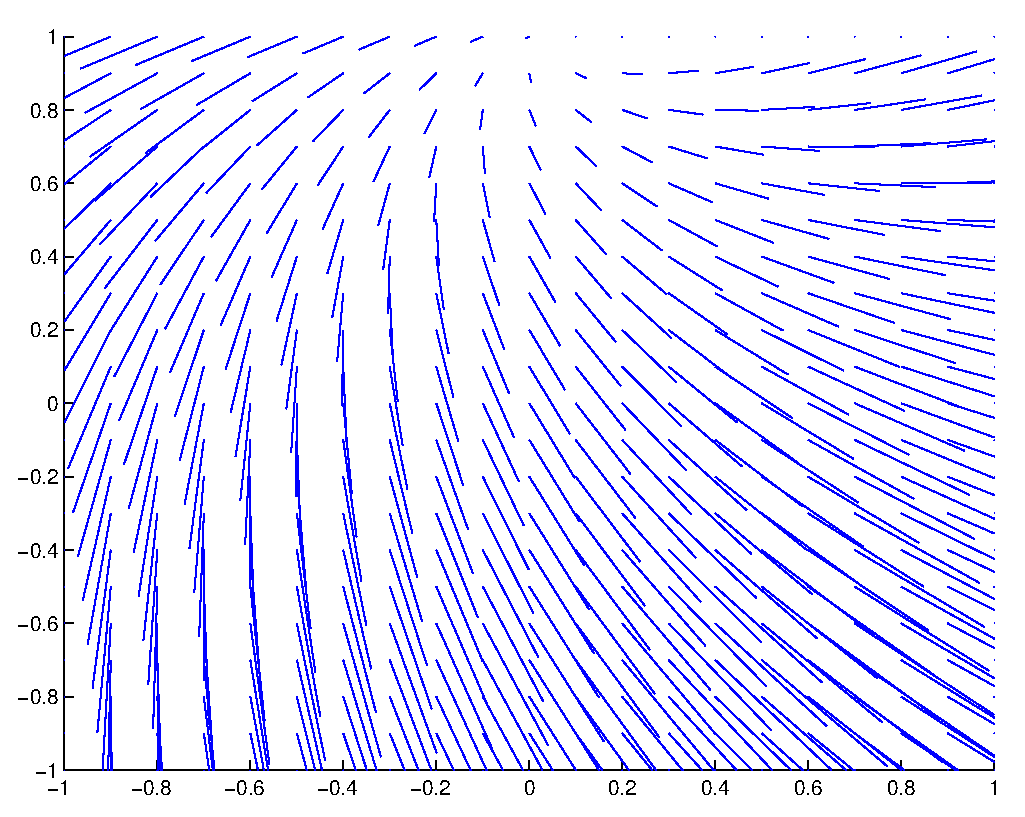
\includegraphics[width = 2in]{stuff}
  \caption[Example small width figure]{
Example small width figure, showing how to use the width option.}
%
  \label{fig:intro_stuff2}
\end{figure}

\begin{figure}[t]
  \centering
  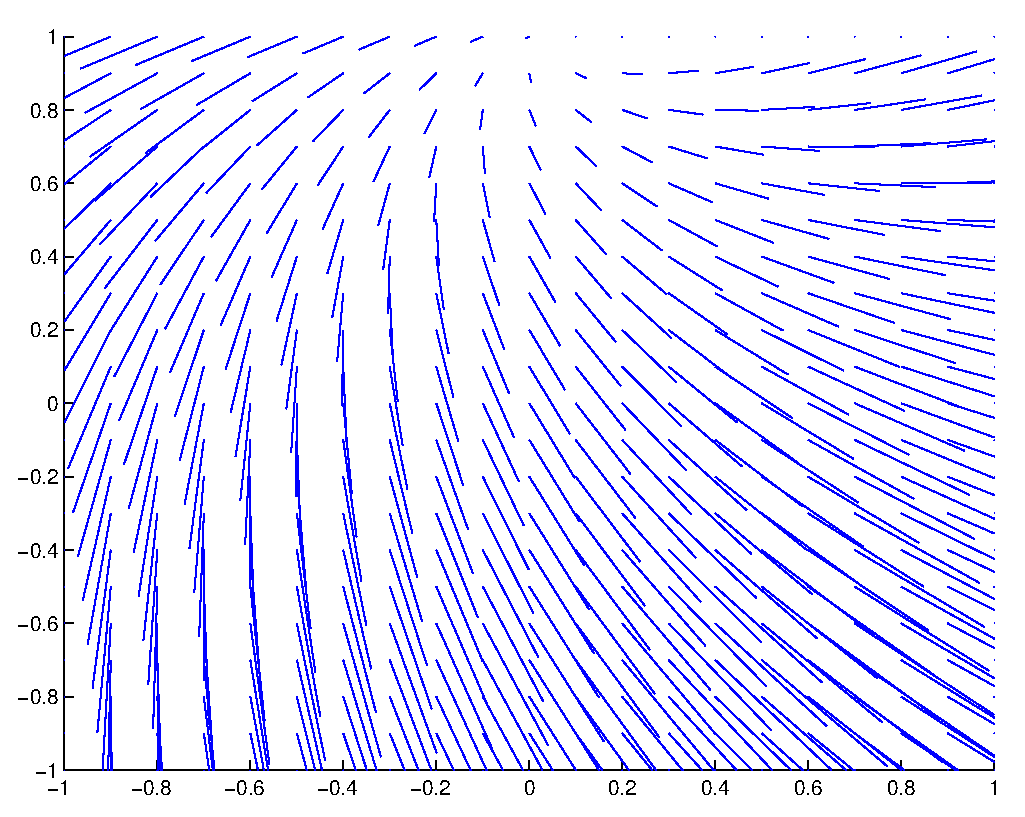
\includegraphics[width=5.5in]{stuff}
  \caption[Example fixed width figure]{
This figure is just a simple figure with a width set at 5.5~in. An example of a
figure whose size depends on the width of the page is given in
Figure \ref{fig:appendix_some_pic} in Section~\ref{sec:appendixa_figure_example} of Appendix~\ref{apdx:appendixa}.}
%
  \label{fig:intro_stuff}
\end{figure}

%\begin{sidewaysfigure}[p]
%\includegraphics[scale=0.8]{examplegraphic}
%\caption{An example of a landscape graphic.}
%\label{fig:example}
%\end{sidewaysfigure}

\section{Math and Equation Example, Where the Heading Is Made so Long That It Extends onto a Second Line}
Here is how to use inline math mode to define lambda like this,
$\lambda$, and how to declare Equations~\eqref{eqn:definition_Ix}
and~\eqref{eqn:definition_Iy}

\begin{equation} \label{eqn:definition_Ix}
I_x(x,y) = \pd{I(x,y)}{x},
\end{equation}

\begin{equation}\label{eqn:definition_Iy}
I_y(x,y) = \pd{I(x,y)}{y}.
\end{equation}

 Or you can create equation arrays like
\begin{align}
  \alpha &= \beta^\gamma \\
  x &= \frac{1}{\alpha} \label{eq:cool_1} \\
  y &= \sqrt{\abs{\frac{\gamma}{\beta}}}  \\
  \zeta &= x^y \label{eq:cool_2}.
\end{align}


The lines in the array can be referenced by saying things like: In
Eqn.~\eqref{eq:cool_1} we show a wonderful equation, but it's not nearly as
amazing as Eqn.~\eqref{eq:cool_2}.

%\chapter{Making Tables}
\label{chp:chapter2}
\graphicspath{{figures/}{figures/chapter2/}}

\section{Making a Table}
An example \LaTeX\ table is shown below in Table~\ref{tab:comparison}.
You make a table by starting a table environment with a caption
and label.  You can specify the text that shows up in the Table of
Contents using the optional parameter box, [], that's at the
beginning of the $\backslash$caption command. You tell the table how
many columns in the beginning of the tabular environment using a
command like this: $|$ l $|$ c $|$ r $|$. That would create a table with 3 columns
that are left-aligned, centered and right-aligned, in that order. The $|$'s tell \LaTeX\ that
you want bars separating the columns. Of course, you can also make tables without the $|$ characters, in which case no lines will be added between the fields, which often looks better. You can also add horizontal
lines using the $\backslash$hline command. This example is also centered in the page using the
$\backslash$centering command.
%
\begin{table}[b]
\centering
\savebox{\tempbox}{
%
\begin{tabular}{|l|c|c|r|}
\hline

Table Name  & Column 2 & Column 3   & Column 4 \\
\hline
First Row   & 4780286  & 72.941376  & A \\
Second Row  & 4069335  & 62.093124  & B \\
Third Row   & 4074900  & 62.178040  & C \\
\hline
Fourth Row  & 4000000  & 60.000000  & Z \\
\hline

\end{tabular}}
% set width
\ifdim\wd\tempbox<\TPTminimum\relax \tempwidth=\TPTminimum\relax
\else\tempwidth=\wd\tempbox
\fi
% format
\begin{minipage}{\tempwidth}\centering
\caption[Example table]{Description of the table, where the caption is long enough to go onto more than one line. The table caption should not extend beyond the edges of the table, and should make an ``inverted pyramid.''}
\label{tab:comparison}
\usebox{\tempbox}
%\end{threeparttable}
\end{minipage}
\end{table}
%

Landscape tables can also be inserted, if desired, using the \verb-sidewaystable- environment, which is defined in the \verb!rotating! package. An example is found on the next page, in Table~\ref{tab:landscape}. Note that landscape tables and figures should be the exception rather than the rule, since they are more awkward to read. However, if you have an especially wide table or figure that cannot be reduced in size without losing required resolution, placing it in landscape may be a good idea.
\begin{sidewaystable}
\centering
\savebox{\tempbox}{
\setlength{\tabcolsep}{6mm}
\begin{tabular}{lcccc}
Year & Method of CVD Deposition & Thickness ($\mu$m) & Hardness (MPa) & Resistivity ($\Omega\cdot$m)\\ 
\hline\\[-11pt]
1999 & LPCVD & 5.1 & 175 & 2.3$\times10^{-5}$\\
2000 & PECVD & 17.2 & 101& 1.5$\times10^{-5}$\\
2002 & PECVD & 4.3 & 55 & 3.4$\times10^{-5}$\\
2004 & LPCVD & 1.1 & 225 & 5.1$\times10^{-5}$\\
\hline
\end{tabular}}
% set width
\ifdim\wd\tempbox<\TPTminimum\relax \tempwidth=\TPTminimum\relax
\else\tempwidth=\wd\tempbox
\fi
% format
\begin{minipage}{\tempwidth}\centering
\caption{A landscape table}\vspace*{6pt}
\label{tab:landscape}
\usebox{\tempbox}
%\end{threeparttable}
\end{minipage}
\end{sidewaystable}
\chapter{Introduction}
\section{Multipath in Aeronautical Telemetry}
Multipath interference is one of the dominant causes for link loss in aeronautical telemetry.
Strong multipath interference occurs in aeronautical telemetry when the transmitted signal is received from multiple paths because a test article is in a low elevation angle scenario as shown in Figure \ref{fig:multipath}.
Multipath propagation is modeled as linear, time-invariant system with a finite impulse response.
Equalizers have been studied to combat multipath interference in aeronautical telemetry \cite{rice-afran-saquib:2014,rice-afran-saquib-cole-rhodes-moazzami:2014}.

There are two types of equalizers, blind and data-aided.
Blind equalizers combat multipath using known properties of the transmitted signal but no knowledge of the data or multipath channel.
Data-aided equalizers require knowing something about the received signal.
One method of providing data that can be used in data-aided equalization is for the transmitter to periodically insert a known bit sequence called a ``pilot'' into the data stream.
The receiver compares the received signal with a locally stored copy to estimate parameters such as multipath channels, frequency offsets, phase offsets and noise variance.
Data-aided equalizers are finite-length impulse response (FIR) filters. The impulse response of the equalizer filter is computed based on the estimated channel better mitigate multipath.
\begin{figure}
	\centering\includegraphics[width=12.11in/100*50]{figures/intro/Picture1.jpg}
	\caption{Multipath can occur when a signal is received multiple paths like line-of-sight or ground bounce or reflections.}
	\label{fig:multipath}
\end{figure}
\section{Problem Statement}
The signal processing for a digital communications system with data-aided equalizers is computationally heavy.
Algorithms implemented in a high powered Central Processing Unit (CPU) can not processing in real-time.
Graphic Processing Units (GPUs) can be used to perform real-time processing because of their massively parallel architecture.

This thesis studies how signal processing can be reformulated to run quickly and efficiently in GPUs.
Processing signals in batches to introduce more parallelism.
Optimized libraries harness GPU resources to make signal processing implementation relatively easy and extremely fast.
If algorithms can be reformulated to used matrix/vector multiplication, solving linear systems of equations, or the Fast Fourier Transform, GPUs can provide vast speed ups.

\section{Organization}
Chapter \ref{chap:equations} shows the equations for these block diagrams.
Chapter \ref{chap:gpu} will shed some light on signal processing in GPUs.
Chapter \ref{chap:equalizers_in_gpus} will illustrate how the five equalizers are implemented in GPUs.
Chapter \ref{chap:final_summary} will summarize.
%%%%%%%%%%%%%%%%%%%%%%%%%%%%%%%%%%%%%%%%%%%%%%%%%%%%%%%%%%%%%%%%%%%%%%%%%%%%%%%%%%%%%%%%%%%%%%
%%%%%%%%%%%%%%%%%%%%%%%%%%%%%%%%%%%%%%%%%%%%%%%%%%%%%%%%%%%%%%%%%%%%%%%%%%%%%%%%%%%%%%%%%%%%%%
%%%%%%%%%%% systemOverview
%%%%%%%%%%%%%%%%%%%%%%%%%%%%%%%%%%%%%%%%%%%%%%%%%%%%%%%%%%%%%%%%%%%%%%%%%%%%%%%%%%%%%%%%%%%%%%
%%%%%%%%%%%%%%%%%%%%%%%%%%%%%%%%%%%%%%%%%%%%%%%%%%%%%%%%%%%%%%%%%%%%%%%%%%%%%%%%%%%%%%%%%%%%%%


% \cleardoublepage
\chapter{PAQ Project}
\label{chap:PAQ_project}
Data-aided equalization in aeronautical telemetry has been studied and tested by the Preamble Assisted Equalization (PAQ) project \cite{paq-phase1-report:2014}.
Under PAQ, a system was built that compared five data-aided equalizers to blind equalization and no equalization.
Laboratory tests were performed using a static RF multipath channel emulator and a noise source to produce bit error rate (BER) curves.
The five data-aided equalizers studied are:
\begin{itemize}
\item zero-forcing (ZF) equalizer,
\item minimum mean-square error (MMSE) equalizer,
\item MMSE-initialized constant modulus algorithm (CMA) equalizer,
\item frequency domain equalizer one (FDE1), and
\item frequency domain equalizer two (FDE2).
\end{itemize}
Bit error rate statistics were used as the figure or merit for the equalization algorithms.
\begin{figure}
	\centering\includegraphics[width=12.33in/100*50]{figures/intro/received1.pdf}
	\caption{The received signal has multipath interference, frequency offset, phase offset, and additive white Gaussian noise. The received signal is down-converted, filtered, sampled, and resampled to produce the sample sequence $r(n)$.}
	\label{fig:received1}
\end{figure}

\section{System Overview}
The system is summarized by the block diagram in Figure \ref{fig:received1}.
%The bit stream $\mathbf{b}$ modulates a SOQPSK-TG carrier.
To enable data-aided equalization, the PAQ bit stream has a packetized structure shown in Figure \ref{fig:packetStructure_intro}. 
Each packet comprises a preamble (defined in the iNET standard \cite{inet-ran:2012}), 
the attached sync marker (ASM), and a $6144$-bit data field. The preamble and ASM bits
form a known sequence of bits, together called the pilot bits, that are periodically inserted every $6144$ bits.
The iNET preamble comprises eight repetitions of the 16-bit sequence $\text{CD98}_\text{hex}$ and the ASM field is
\begin{equation}
\text{034776C7272895B0}_\text{hex}.
\end{equation}
The data payload is a known length-$(2^{11} - 1)$ PN sequence.
Each packet contains $128$ preamble bits, $64$ ASM bits and $6{,}144$ data bits making each iNET packet $6{,}336$ bits.
The data bit rate is $10$ Mbits/s. 
After preamble and ASM insertion, the bit rate presented to the modulator is $10.3125$ Mbits/s.

After modulation, the transmitted signal experiences multipath interference modeled as an LTI system with the channel impulse response $h(t)$.
The transmitted signal also experiences a frequency offset $\omega_0$, a phase offset $\phi$ and additive white Gaussian noise $w(t)$.
The received signal is down-converted, filtered, sampled at $93\nicefrac{1}{3}$ Msamples/second by the ADC, and down-converted to baseband and resampled by $\nicefrac{99}{448}$ using a polyphase filterbank based on the principles outlined in \cite[chap. (9)]{rice:2009}.
The result is $r(n)$, a sampled version of the complex-valued lowpass equivalent waveform at a sample rate of $20.625$ Msamples/second or $2$ samples/bit.
\begin{figure}
	\centering\includegraphics[width=9.47in/100*55]{figures/intro/packetSturcture.pdf}
	\caption{A diagram showing each PAQ packet comprises a preamble, ASM, and a data field.}
	\label{fig:packetStructure_intro}
\end{figure}

\section{Hardware Overview}
\label{sec:hardware}
A block diagram of PAQ physical system is shown in Figure \ref{fig:hardwareblock}.
\begin{figure}
	\centering\includegraphics[width=11.58in/100*55]{figures/systemOverview/hardwareblock.pdf}
	\caption{A block diagram of the physical PAQ hardware. The components inside the rack mounted server are in the dashed box. All the components in the dashed and dotted box are housed in a rack mounted case.}
	\label{fig:hardwareblock}
\end{figure}
A picture of the physical components is shown in Figure \ref{fig:HostSystem}.
\begin{figure}
	\centering\includegraphics[scale=0.55]{figures/systemOverview/HostSystem.jpg}
	\caption{A picture of the physical PAQ hardware refrencing blocks from Figure \ref{fig:hardwareblock}. Right: Components in the dashed and dotted box. Left: Components in the dashed box. Note that the T/M Receiver is not pictured.}
	\label{fig:HostSystem}
\end{figure}
The major components, and their functions are summarized as follows:
\begin{itemize}
	\item The \textbf{T/M receiver} down-converts the received signal from L- or C-band RF to 70 MHz IF.
	The IF filter plays the role of an anti-aliasing filter.
	%
	\item The \textbf{ADC} produces 14-bit samples of the real-valued bandpass IF signal.
	The sample rate is $93\nicefrac{1}{3}$ Msamples/s.
	The samples are transferred to the host CPU via the PCIe bus.
	%
	\item The \textbf{host CPU} initiates memory transfers between itself and the ADC, GPUs and FPGA via the PCIe 	bus. 
	The host CPU also launches the digital signal processing algorithms on the GPUs.
	%
	\item The three \textbf{GPUs} are where the detection, estimation, equalization and demodulation resides.
%	While the CPU has one to eight powerful processors, GPUs have thousands of small less powerful processors that work in parallel. The signal processing is done in GPUs rather than FPGAs or a CPU because programming GPUs is faster and easier than programming FPGAs and CPUs do not prosess the required processing power.
	%
	\item The bit error rate tester (\textbf{BERT}) counts the errors in each bit stream by comparing the 		streams to the transmitted PN sequence.
	%
	\item The \textbf{FPGA} is the interface between the host CPU and the BERT. After the GPUs produce bit decisions, the host CPU transfers the decisions from the GPUs to the FPGA via the PCIe bus. The FPGA then clocks the bits out to the BERT for BER testing.
	%
	\item The \textbf{T/M Receiver \& Demodulator} demodulates the RF signal outputting two bit streams for blind equalization and no equalization for BER comparison.
	%
	\item The \textbf{rack mounted server} is a high powered computer that houses an ADC, a FPGA and three GPUs 			slotted into a 32 pin PCIe bus.
\end{itemize}
%A picture of the rack mounted physical system is shown in Figure \ref{fig:rack}.
%\begin{figure}
%	\centering\includegraphics[scale=0.55]{figures/systemOverview/rack.jpg}
%	\caption{A picture of the physical PAQ hardware. Note that the T/M Receiver is not pictured.}
%	\label{fig:rack}
%\end{figure}
%A picture of the components inside the rack mounted server is shown in Figure \ref{fig:rack}.
%\begin{figure}
%	\centering\includegraphics[scale=0.55]{figures/systemOverview/server.jpg}
%	\caption{A pictureof the components inside the rack mounted server.}
%	\label{fig:server}
%\end{figure}

\section{Digital Signal Processing}
\label{sec:signalProcessing}
A high-level digital signal processing flow and notation is shown in Figure \ref{fig:fullSystem}.
The sequence $r(n)$ represents a continuous stream of samples.
Because the frequency offset, channel, and noise variance are estimated using the preamble and ASM, the first step is to find the samples corresponding to the preamble in the received sample sequence $r(n)$.
The preamble detector identifies the sample indices in the sequence $r(n)$ corresponding to the starting position of each occurrence of the waveform samples corresponding to the preamble.
To simplify the notation used to describe the signal processing algorithms, we represent the output of the preamble detector by the vector $\mathbf{r}_\text{p}$, a sequence of $\Lpkt$ samples starting with the waveform samples corresponding to the preamble and ASM bits.
In this way the signal processing algorithms are described on a packet-by-packet basis.

Starting with the block diagram in Figure \ref{fig:fullSystem}, the preamble samples are used first to estimate the frequency offset.
The estimated frequency offset $\hat{\omega}_0$ rads/sample is then used to ``de-rotate'' the vector of samples $\mathbf{r}_\text{p}$ to produce a vector denoted $\tilde{\mathbf{r}}$.
The de-rotated preamble and ASM samples in the vector $\tilde{\mathbf{r}}$ are used to estimate the channel $\hat{\mathbf{h}}$ and noise variance $\hat{\sigma}^2_w$ as shown.
\begin{sidewaysfigure}
	\includegraphics[width=15.72in/100*55]{figures/eq_equations/fullSystem.pdf}
	\caption{A block diagram of the digital signal processing flow and notation in PAQ.}
	\label{fig:fullSystem}
\end{sidewaysfigure}
%\begin{figure}
%	\centering\includegraphics[width=8.75in/100*55]{figures/intro/estimators.pdf}
%	\caption{A block diagram of the estimators in PAQ.}
%	\label{fig:estimators}
%\end{figure}

The estimates are used to compute the equalizer filter coefficients as illustrated in Figure \ref{fig:thisThesisBlock}.
The figure shows five independent branches,
each branch computing an equalizer filter.
On the top three branches, lower case boldface variables $\mathbf{c}$, with a subscript, represent the impulse responses of the FIR equalizer filters. 
On the lower two branches, the upper case boldface $\mathbf{C}$ with a subscript represent the FFT-domain transfer function of the equalizers.
In all five cases, the equalizer and a detection filter (described below) are applied to $\tilde{\mathbf{r}}$.
The result processed by a symbol-by-symbol OQPSK detector to produce bit decisions for each equalizer.
\begin{figure}
	\centering\includegraphics[width=10.45in/100*55]{figures/intro/thisThesisBlock5.pdf}
	\caption{A block diagram of the computation and application of the equalizer and detection filters. The bold box emphasizes the focus of this thesis.}
	\label{fig:thisThesisBlock}
\end{figure}

The GPUs in Figure \ref{fig:hardwareblock} and \ref{fig:HostSystem} perform all the digital signal processing in parallel.
To introduce as much parallelism as possible, the received samples are processed in a batch comprising $39{,}321{,}600$ samples. 
At $20.625$ Msamples/second, each batch of $39{,}321{,}600$ samples represents $1907$ milliseconds of data.
Each batch has at most $3104$ $12{,}672$-sample iNET packets.%
\footnote{Because the batch length ($39{,}321{,}600$ samples) is not a multiple of the packet length ($12{,}672$), each batch comprises $3103$ or $3104$ packets.}
The GPU processes $3104$ packets in parallel by leveraging batched processing.
To meet the real-time requirement, all processing must be completed in less than $1907$ ms.

This thesis illustrates how the five PAQ data-aided equalizers were computed and applied in GPUs.
The bold box in Figure \ref{fig:thisThesisBlock} emphasizes processing blocks on which this thesis focuses.
Even though the GPUs process $3104$ packets in parallel, the signal processing algorithms are described on a
packet-by-packet basis.

\subsection{Preamble Detection}
\label{sec:pd}
To compute the impulse responses or transfer functions of the five data-aided equalizers, an estimate of the channel and noise variance must be available.
The required estimates are derived from the received waveform samples corresponding to the preamble and ASM bits.
Consequently, the location of the waveform samples corresponding to the preamble and ASM bits must be found.
The preamble detector identifies the sample indices in the sequence $r(n)$ corresponding to the starting position of each occurrence of the waveform samples corresponding to the preamble.
The preamble detector computes the function $L(n)$ for each sample in the batch.
Peaks in $L(n)$ identify the starting indices of the waveform samples corresponding to each occurrence of the preamble bits.
The function $L(n)$ is given by \cite{preamble_detector}
\begin{equation}
	L(n) = \sum_{m=0}^{7}
		\left[ I^2(n,m) + Q^2(n,m) \right],
	\label{eq:gpu-L-4}
\end{equation}
where
\begin{multline}
	I(n,m) \approx \sum_{\ell\in\mathcal{L}_1}r_R(\ell+32m+n)
			- \sum_{\ell\in\mathcal{L}_2}r_R(\ell+32m+n)
			+ \sum_{\ell\in\mathcal{L}_3}r_I(\ell+32m+n)
			- \sum_{\ell\in\mathcal{L}_4}r_I(\ell+32m+n)
			\\
			+ 0.7071 \left[
				\sum_{\ell\in\mathcal{L}_5}r_R(\ell+32m+n)
				- \sum_{\ell\in\mathcal{L}_6}r_R(\ell+32m+n)
			\right. \\
			\left.
				+ \sum_{\ell\in\mathcal{L}_7}r_I(\ell+32m+n)
				- \sum_{\ell\in\mathcal{L}_8}r_I(\ell+32m+n)
			\right],
	\label{eq:gpu-L-pedone-geoghegan-2}
\end{multline}
and
\begin{multline}
	Q(n,m) \approx \sum_{\ell\in\mathcal{L}_1}r_I(\ell+32m+n)
			- \sum_{\ell\in\mathcal{L}_2}r_I(\ell+32m+n)
			\\
			- \sum_{\ell\in\mathcal{L}_3}r_R(\ell+32m+n)
			+ \sum_{\ell\in\mathcal{L}_4}r_R(\ell+32m+n)
			\\
			+ 0.7071 \left[
				\sum_{\ell\in\mathcal{L}_5}r_I(\ell+32m+n)
				- \sum_{\ell\in\mathcal{L}_6}r_I(\ell+32m+n)
			\right. \\
			\left.
				- \sum_{\ell\in\mathcal{L}_7}r_R(\ell+32m+n)
				+ \sum_{\ell\in\mathcal{L}_8}r_R(\ell+32m+n)
			\right],
		\label{eq:gpu-L-pedone-geoghegan-3}
\end{multline}
with
\begin{equation}
	\begin{split}
	\mathcal{L}_1 &= \{ 0, 8, 16, 24 \}\\
	\mathcal{L}_2 &= \{ 4, 20 \}\\
	\mathcal{L}_3 &= \{ 2, 10, 14, 22 \}\\
	\mathcal{L}_4 &= \{ 6, 18, 26, 30 \}\\
	\mathcal{L}_5 &= \{ 1, 7,  9, 15, 17, 23, 25, 31 \}\\
	\mathcal{L}_6 &= \{ 3, 5, 11, 12, 13, 19, 21, 27, 28, 29 \}\\
	\mathcal{L}_7 &= \{ 1, 3,  9, 11, 12, 13, 15, 21, 23 \}\\
	\mathcal{L}_8 &= \{ 5, 7, 17, 19, 25, 27, 28, 29, 31 \}.
\end{split}
\label{eq:gpu-L-pedone-geoghegan-4}
\end{equation}
The index of a peak in $L(n)$ indicates the start of a preamble.
Suppose $L(i)$ is a peak (i.e., $i$ is the index of the peak).
Then the vector $\mathbf{r}_\text{p}$ in Figure \ref{fig:fullSystem} is 
\begin{equation}
\mathbf{r}_\text{p} = 
\begin{bmatrix}
r(i) \\ 
\vdots \\ 
r(i+\Lpkt-1)
\end{bmatrix}
=
\begin{bmatrix}
r_\text{p}(0) \\ 
\vdots \\ 
r_\text{p}(\Lpkt-1)
\end{bmatrix}.
\end{equation}
The first $L_\text{p} = 256$ samples of $\mathbf{r}_\text{p}$ correspond to the preamble bits and the following
$L_\text{ASM} = 128$ samples of $\mathbf{r}_\text{p}$ correspond to the ASM bits.


\subsection{Frequency Offset Compensation}
\label{sec:freq_offset_comp}
The preamble sequence comprises eight copies of the bit sequence CD98\textsubscript{hex}.
Consequently, the waveform samples $r_\text{p}(0), \ldots , r_\text{p}(L_\text{p}-1)$ comprise 
eight copies of $L_q=32$ SOQPSK-TG waveform samples corresponding to CD98\textsubscript{hex}.%
\footnote{This statement is only approximately true. 
Because of the memory in SOQPSK-TG, the first block of $L_q$ samples is a function of both the bit sequence CD98\textsubscript{hex} and the seven unknown bits preceding the first occurrence of CD98\textsubscript{hex}.}
The frequency offset estimator shown in Figure \ref{fig:fullSystem} is the estimator taken from \cite[eq. (24)]{rice2014frequency}.
With the notation adjusted slightly, the frequency offset estimate is
\begin{equation}
	\hat{\omega}_0 = \frac{1}{L_q} \arg\left\{ \sum_{n=i+2L_q}^{i+7L_q-1} r_\text{p}(n)r_\text{p}^\ast(n-L_q)\right\}
	\quad
\text{for} \;
i=1,2,3,4,5.
	\label{eq:jeff-ML-w-final3}
\end{equation}
The frequency offset is estimated for every packet or each vector of samples $\mathbf{r}_\text{p}$ in the batch.
Frequency offset compensation is performed by de-rotating the received samples by $-\hat{\omega}_0$:
\begin{equation}
	\tilde{r}(n) = r_\text{p}(n) e^{-j\hat{\omega}_0n}.
	\label{eq:frequency_compensation}
\end{equation}
Equations \eqref{eq:jeff-ML-w-final3} and \eqref{eq:frequency_compensation} are easily implemented into GPUs. 

\subsection{Channel Estimation}
\label{sec:channel_estimation}
Let the SOQPSK-TG samples corresponding to the preamble and ASM bits be
\begin{equation}
\mathbf{p} = 
\begin{bmatrix}
p(0) \\
p(1) \\
\vdots \\
p(L_\text{P} + L_\text{ASM}-1)
\end{bmatrix}.
\label{eq:preamble_ASM}
\end{equation}
The multipath channel is defined by the impulse response 
\begin{equation}
\mathbf{\hat{h}} = 
\begin{bmatrix}
\hat{h}(-N_1) \\ \vdots \\ \hat{h}(0) \\ \vdots \\ \hat{h}(N_2)
\end{bmatrix}.
\end{equation}
Note that at $2$ samples/bit, the complex-valued lowpass equivalent channel impulse response is assumed to have a non-causal component comprising $N_1$ samples and a causal component comprising $N_2$ samples.
Figure \ref{fig:channelExample} shows the full discrete-time $L_h = N_1+N_2+1$ sample channel.
\begin{figure}
	\centering\includegraphics[width=5.5in/100*55]{figures/intro/channelExample.pdf}
	\caption{An illustration of the discrete-time channel of length $N_1+N_2+1$ with a non-causal component comprising $N_1$ samples and a causal component comprising $N_2$ samples.}
	\label{fig:channelExample}
\end{figure} \newline
The ML estimate is \cite[eq. 8]{rice-afran-saquib-cole-rhodes-moazzami:2014} 
\begin{equation}
\hat{\mathbf{h}} = \underbrace{ \left( \mathbf{X}^\dag\mathbf{X} \right)^{-1} \mathbf{X}^\dag}_{\mathbf{X}_\text{lpi}}\tilde{\mathbf{r}}_x,
\end{equation}
where 
\begin{equation}
\mathbf{X} = 
		\begin{bmatrix}
		p(N_2)							& 								& 		&  			\\
		\vdots 							& p(N_2)						& 		&  			\\
		p(L_\text{p}+L_\text{ASM}-N_1)	&\vdots							& \ddots&  			\\
										& p(L_\text{p}+L_\text{ASM}-N_1)&  		& p(N_2)  	\\
		 								&  								&  		& \vdots 	\\
		 								&  	   							&  		& p(L_\text{p}+L_\text{ASM}-N_1)\\
	\end{bmatrix},
	\label{eq:X}
\end{equation}
is the $(L_\text{p}+L_\text{ASM}-N_1-N_2)\times(N_1+N_2+1)$ convolution matrix formed from 
the SOQPSK-TG waveform samples corresponding to the preamble and ASM bits and $\tilde{\mathbf{r}}_x$ is the vector of de-rotated received waveform samples corresponding to the ``middle'' portion of the preamble and ASM bits:
\begin{equation}
\tilde{\mathbf{r}}_x = 
\begin{bmatrix}
\tilde{r}(N_2) \\
\tilde{r}(N_2+1) \\
\vdots \\
\tilde{r}(L_\text{P} + L_\text{ASM}-N_1)
\end{bmatrix}.
\label{eq:r_x}
\end{equation}
The $(N_1+N_2+1)\times(L_\text{p}+L_\text{ASM}-N_1-N_2)$ matrix $\mathbf{X}_\text{lpi}$ is the left pseudo-inverse of $\mathbf{X}$.
Note that $\mathbf{X}_\text{lpi}$ is independent of the data and therefore may be computed once and stored.
The matrix vector multiplication $\mathbf{X}_\text{lpi} \tilde{\mathbf{r}}_x$ is implemented simply and efficiently in GPUs.


\subsection{Noise Variance Estimation}
\label{sec:noise_variance_estimation}
The noise variance estimator is \cite[eq. 9]{rice-afran-saquib-cole-rhodes-moazzami:2014}
\begin{equation}
	\hat{\sigma}_w^2 = \frac{1}{2\rho} \left| \tilde{\mathbf{r}}_x-\mathbf{X}\hat{\mathbf{h}}\right|^2,
	\label{eq:ML-s2-final3}
\end{equation}
where
\begin{equation}
	\rho = {\rm Trace} \left\{ \mathbf{I} -  \mathbf{X}\left(\mathbf{X}^\dag\mathbf{X}\right)^{-1}\mathbf{X}^\dag \right\},
\end{equation}
where $\tilde{\mathbf{r}}_x$ is given by Equation \eqref{eq:r_x} and $\mathbf{X}$ is given by Equation \eqref{eq:X}.
Equation \eqref{eq:ML-s2-final3} is easily implemented into GPUs.

\subsection{Equalizers}
\label{sec:equalizer_eq}

\subsubsection{Zero-Forcing Equalizer}
The ZF equalizer is an FIR filter defined by the $L_\text{eq}=L_1+L_2+1$ coefficients
\begin{equation}
\mathbf{c}_\text{ZF} = 
\begin{bmatrix}
c_\text{ZF}(-L_1) \\ \vdots \\ c_\text{ZF}(0) \\ \vdots \\ c_\text{ZF}(L_2)
\end{bmatrix}.
\end{equation}
The filter coefficients are the solution to \cite{paq-phase1-report:2014}
\begin{equation}
\mathbf{R}_{\hat{h}} \mathbf{c}_\text{ZF} = \hat{\mathbf{g}},
\label{eq:start_here_ZF_MDR}
\end{equation}
where
\begin{equation}
\mathbf{R}_{\hat{h}} = 
		\begin{bmatrix}
		r_{\hat{h}}(0)			& r^\ast_{\hat{h}}(1)	& \cdots 	& r^\ast_{\hat{h}}(L_{eq}-1)  	\\
		r_{\hat{h}}(1) 			& r_{\hat{h}}(0)		& \cdots 	& r^\ast_{\hat{h}}(L_{eq}-2)  	\\
		\vdots	 				& \vdots				& \ddots 	&  								\\
		r_{\hat{h}}(L_{eq}-1)	& r_{\hat{h}}(L_{eq}-2)	& \cdots	& r_{\hat{h}}(0)  			
	\end{bmatrix},
	\label{eq:R_h_MDR}
\end{equation}
\begin{equation}
\hat{\mathbf{g}} = 
\begin{bmatrix} \hat{h}^\ast(L_1) \\ \vdots \\ \hat{h}^\ast(0) \\ \vdots \\ \hat{h}^\ast(-L_2)  \end{bmatrix},
\label{eq:g_MDR}
\end{equation}
and
\begin{equation}
r_{\hat{h}}(k) = \sum_{n=-N_1}^{N_2} \hat{h}(n) \hat{h}^\ast(n-k).
\label{eq:sample_autocorrelation_ZF_MDR}
\end{equation}

\subsubsection{MMSE Equalizer}
The MMSE equalizer is an FIR filter defined by the $L_\text{eq}=L_1+L_2+1$ coefficients
\begin{equation}
\mathbf{c}_\text{MMSE} = 
\begin{bmatrix}
c_\text{MMSE}(-L_1) \\ \vdots \\ c_\text{MMSE}(0) \\ \vdots \\ c_\text{MMSE}(L_2)
\end{bmatrix}.
\end{equation}
The filter coefficients are the solution to \cite{paq-phase1-report:2014}
\begin{equation}
\mathbf{R} \mathbf{c}_\text{MMSE} = \hat{\mathbf{g}},
\label{eq:start_here_MMSE_MDR}
\end{equation}
where
\begin{equation}
\mathbf{R} = 
\mathbf{R}_{\hat{h}} + \hat{\sigma}^2_w \mathbf{I},
\end{equation}
$\mathbf{R}_{\hat{h}}$ is given by \eqref{eq:R_h_MDR}, $\hat{\sigma}^2_w$ is given by \eqref{eq:ML-s2-final3}, and $\hat{\mathbf{g}}$ is given by \eqref{eq:g_MDR}.

\subsubsection{Constant Modulus Algorithm Equalizer}
The CMA equalizer is an adaptive FIR filter where the $L_\text{eq}=L_1+L_2+1$ coefficients at the $b$-th iteration are
\begin{equation}
\mathbf{c}_\text{CMA}^{(b)} = 
\begin{bmatrix}
c_\text{CMA}^{(b)}(-L_1) \\ \vdots \\ c_\text{CMA}^{(b)}(0) \\ \vdots \\ c_\text{CMA}^{(b)}(L_2)
\end{bmatrix}.
\end{equation}
The equalizer output at the $b$-th iteration is 
\begin{equation}
\hat{\mathbf{s}}^{(b)} = 
\mathbf{c}_\text{CMA}^{(b)} \ast \tilde{\mathbf{r}}.
\end{equation}
Note that in this implementation the CMA filter coefficients are constant for the duration of a packet \cite{rice-afran-saquib-cole-rhodes-moazzami:2014}.
The filter coefficients are updated on a packet-by-packet basis using a steepest descent algorithm as follows:
\begin{equation}
\mathbf{c}_\text{CMA}^{(b+1)} = \mathbf{c}_\text{CMA}^{(b)}-\mu \nabla J,
\label{eq:steepest}
\end{equation}
where
\begin{equation}
	\nabla J = \frac{2}{L_{pkt}} \sum_{n=0}^{L_{pkt}-1}
	\left[ \vphantom{\displaystyle\sum}  \hat{s}^{(b)}(n) \left( \hat{s}^{(b)}(n)\right)^\ast - 1 \right]
	\hat{s}^{(b)}(n)  \tilde{\mathbf{r}}^\ast(n).
\label{eq:DelJcma-approxr_MDR}
\end{equation}
In Equation \eqref{eq:DelJcma-approxr_MDR}, $\hat{s}^{(b)}(n)$ is the $n$-th element of the vector $\hat{\mathbf{s}}^{(b)}$ and
\begin{equation}
\tilde{\mathbf{r}}^\ast(n) = \begin{bmatrix} \tilde{r}^\ast(n+L_1) \\ \vdots \\ \tilde{r}^\ast(n) \\ \vdots \\ \tilde{r}^\ast(n-L_2) \end{bmatrix}.
\label{eq:r_tilde_n}
\end{equation}
The CMA equalizer filter coefficients are initialized by the MMSE equalizer filter coefficients
\begin{equation}
\mathbf{c}_\text{CMA}^{(0)} = \mathbf{c}_\text{MMSE}.
\label{eq:CMA_init}
\end{equation}

\subsubsection{Frequency Domain Equalizer One}
Frequency-domain equalization leverages the efficiency of the FFT algorithm to perform equalization filtering in the FFT domain.
The difference between frequency-domain equalization and applying the previous three equalizer filters in the FFT domain is that the frequency-domain equalizer is computed directly in the FFT domain.
To enable this, some provision must be made for the fact that point-by-point multiplication in the FFT domain corresponds to circular convolution in the time domain.
This provision is most often in the form of a cyclic prefix prepended to the data packet \cite{sari1994frequency,ng2007turbo,al2008single,proakis-salehi:2008}.
Even though the PAQ format does not include any special provision for frequency-domain equalization such as a cyclic prefix, frequency-domain equalization is still possible using the ideas described by Coon et al \cite{coon-sandell-beach-mcgeehan:2006}.
Because of the repetitive nature of the preamble sequence, the second half of the preamble bits at the beginning of the packet are the same the first half of the preamble bits following the packet.
Consequently, the second half of the preamble bits at the beginning of the packet form a cyclic prefix for the block comprising the ASM, the data, and the first half of the preamble following the packet as illustrated in Figure \ref{fig:cyclicPrefix_MDR}.
\begin{figure}
	\centering\includegraphics[width=10.63in/100*55]{figures/eq_equations/cyclicPrefix.pdf}
	\caption{A diagram showing how the iNET packet is used as a cyclic prefix.}
	\label{fig:cyclicPrefix_MDR}
\end{figure}

The FFT domain transfer function of FDE1 is \cite[eq. (11)]{williams2013linear}
\begin{equation}
C_\text{FDE1}(e^{j\omega_k}) = \frac{\hat{H}^\ast(e^{j\omega_k})}  {|\hat{H}(e^{j\omega_k})|^2  +  \frac{1}{\hat{\sigma}^2_w}} \quad
\omega_k = \frac{2\pi}{N_\text{FFT}} \;
\text{for} \;
k=0,1,\cdots,N_\text{FFT}-1,
\label{eq:FDE1_MDR}
\end{equation}
where $N_\text{FFT} = 2^u = 16{,}384$, where $u = {\left\lceil \log_2{\left(\Lpkt\right)}  \right\rceil} = 14$,
where $\left\lceil x  \right\rceil$ means the smallest integer greater than or equal to $x$.
In Equation \eqref{eq:FDE1_MDR}, $\hat{H}(e^{j\omega_k})$ is the $k$-th element of the length-$N_\text{FFT}$ FFT of $\mathbf{\hat{h}}$ and $\hat{\sigma}^2_w$ is given by \eqref{eq:ML-s2-final3}.
FDE1 is the MMSE equalizer formulated in the frequency domain, where power spectral density of SOQPSK-TG is a constant.

\subsubsection{Frequency Domain Equalizer Two}
The FFT domain transfer function of FDE1 is \cite[eq. (12)]{williams2013linear}
\begin{equation}
C_\text{FDE2}(e^{j\omega_k}) = \frac{\hat{H}^\ast(e^{j\omega_k})}  {|\hat{H}(e^{j\omega_k})|^2  +  \frac{\Psi(e^{j\omega_k})}{\hat{\sigma}^2_w}} \quad
\omega_k = \frac{2\pi}{N_\text{FFT}} \;
\text{for} \;
k=0,1,\cdots,N_\text{FFT}-1,
\label{eq:FDE2_MDR}
\end{equation}
where $N_\text{FFT} = 2^u = 16{,}384$, where $u = {\left\lceil \log_2{\left(\Lpkt\right)}  \right\rceil} = 14$,
where $\left\lceil x  \right\rceil$ means the smallest integer greater than or equal to $x$.
In Equation \eqref{eq:FDE2_MDR}, $\hat{H}(e^{j\omega_k})$ is the $k$-th element of the length-$N_\text{FFT}$ FFT of $\mathbf{\hat{h}}$ and $\hat{\sigma}^2_w$ is given by \eqref{eq:ML-s2-final3}.
Like FDE1, FDE2 is the MMSE equalizer formulated in the frequency domain.
The difference is FDE2 uses an estimate of the true power spectral density of SOQPSK-TG.
The SOQPSK-TG power spectral density $\Psi(e^{j\omega_k})$ is illustrated in Figure \ref{fig:SOQPSK_spectrum_MDR}.
$\Psi(e^{j\omega_k})$ was estimated using Welch's method of periodogram averaging based on length-$N_\text{FFT} $ FFTs of SOQPSK-TG sampled at $2$ samples/bit, the Blackman window, and $50\%$ overlap.
\begin{figure}
	\centering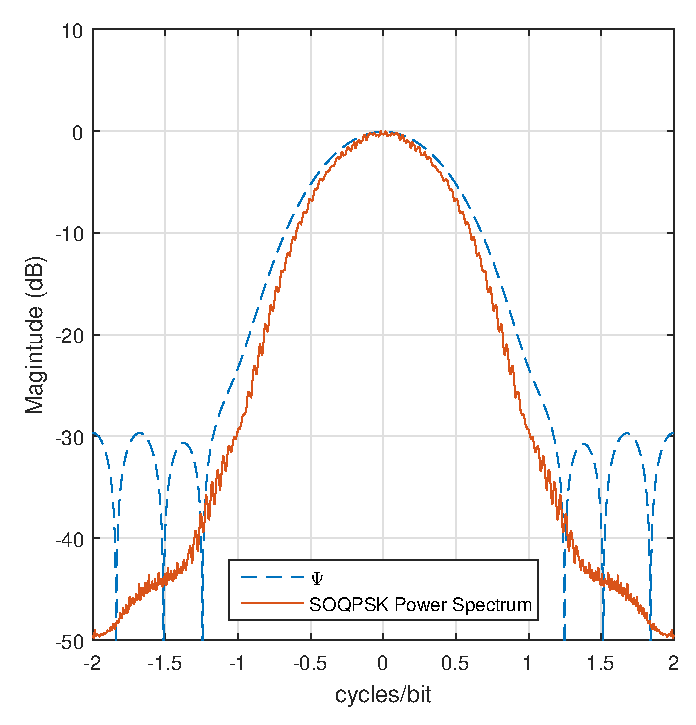
\includegraphics[width=5in]{figures/eq_equations/FDE2_spectrum_PSI.eps}
	\caption{SOQPSK-TG power spectral density.}
	\label{fig:SOQPSK_spectrum_MDR}
\end{figure}

\subsection{Symbol-by-Symbol Detector}
\label{sec:oqpsk_detector}
A block diagram of the symbol-by-symbol detector is shown in Figure \ref{fig:OQPSK}.
Note that the detection filter is applied with the equalizer filter in Figure \ref{fig:thisThesisBlock}.
Symbol-by-symbol detection comprises a detection filter operating at $2$ samples/bit, a phase lock loop (PLL) operating at $1$ sample/bit, and a decision device also operating at $1$ sample/bit.
Before the symbols are detected, the equalized samples $\hat{s}(n)$ are passed through the detection filter then down-sampled by $2$. 
The detection filter $\mathbf{d}$ is the length $L_\text{d} = 23$ FIR filter whose response is shown in Figure \ref{fig:detectionFilter} \cite[Fig. 3]{perrins:2013}.
\begin{figure}
%	\centering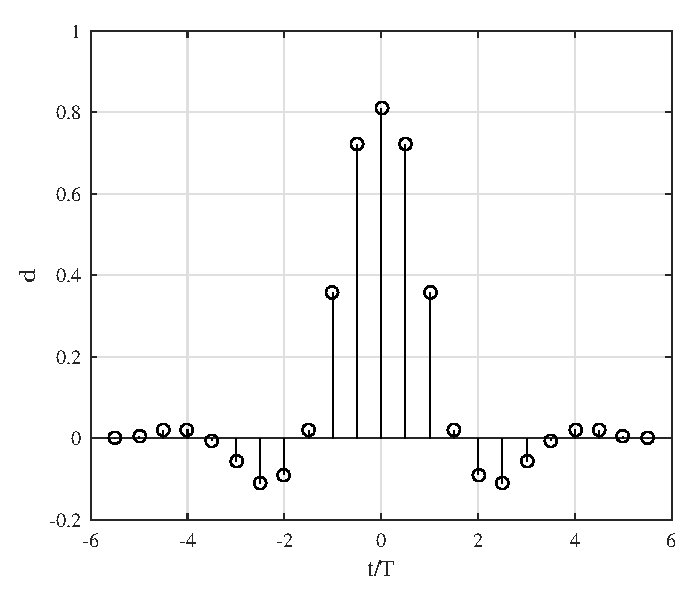
\includegraphics[width=5in]{figures/eq_equations/df.eps}
	\centering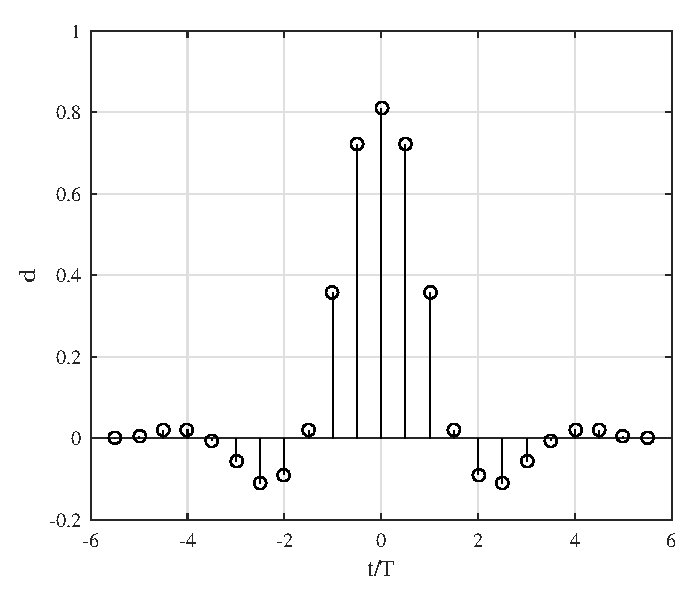
\includegraphics[width=4.25in]{figures/eq_equations/df.eps}
	\caption{SOQPSK detection filter $\mathbf{d}$.}
	\label{fig:detectionFilter}
\end{figure}
The symbol-by-symbol detector block in Figure \ref{fig:thisThesisBlock} is an OQPSK detector.
\begin{figure}
	\centering\includegraphics[width=11.83in/100*55]{figures/systemOverview/OQPSK.pdf}
	\caption{Offset Quadrature Phase Shift Keying symbol-by-symbol detector.}
	\label{fig:OQPSK}
\end{figure}

A phase lock loop (PLL) is needed in the OQPSK detector to track out residual frequency offset.
The residual frequency offset results from a frequency offset estimation error.
Equalizers mitigate the effects of phase offset, timing offset, and ISI because all of these impairments form the  composite channel seen by the equalizer.
A frequency offset is different, and cannot be mitigated by the equalizer alone.
The PLL tracks out the residual frequency offset using a feedback control loop.
The feedback control loop operates in a data-aided mode for $k<L_\text{p}+L_\text{ASM}$ using the known bits of preamble and ASM, denoted $a(k)$ in the figure.
Note that $y(n)$ is indexed at $2$ samples/bit while $y(k)$ and $\tilde{y}(k)$ are indexed at $1$ sample/bit.

Implementing a PLL may not seem feasible in GPUs because the feedback loop cannot be parallelized.
But the PAQ system processes $3104$ packets of data simultaneously in parallel.
Running the PLL and detector serially through a full packet of samples is relatively fast because the loop requires only $10$ floating point operations and a few logic decisions.
\chapter{Signal Processing in GPUs}
\label{chap:gpu}
A graphics processing unit (GPU) is a computational unit with a highly-parallel architecture well-suited for executing the same function on many data elements.
In the past, GPUs were used to process graphics data but in 2008 NVIDIA released the Tesla GPU.
Telsa GPUs are built for general purpose high performance computing.
Figure \ref{fig:GPUpicture} shows the form factor of a Tesla K40c and K20c.
\begin{figure}
	\centering\includegraphics[width=5in]{figures/gpu_intro/k40c_k20c.jpg}
	\caption{NVIDIA Tesla K40c and K20c.}
	\label{fig:GPUpicture}
\end{figure}

In 2007 NVIDIA released an extension to C, C++ and Fortran called CUDA (Compute Unified Device Architecture).
CUDA enables GPUs to be used for high performance computing in computer vision, deep learning, artificial intelligence, and signal processing \cite{wikipedia-gpu:2015}.
CUDA allows a programmer to write C++ like functions that are massively parallel called kernels.
To invoke parallelism, a GPU kernel executed $N$ times with the work distributed to $N_\text{min}$ total threads that run concurrently.
To achieve the full potential of high performance GPUs, kernels must be written with some basic concepts about GPU architecture and memory in mind.
This chapter will show the following:
\begin{itemize}
\item Optimizing memory access leads to faster execution time, rather than optimizing number of floating point operations.
\item The number of threads per block can significantly affect execution time.
\item CPU and GPU processing can be pipelined.
\item Convolution maps very well to GPUs using the Fast Fourier Transform (FFT).
\item Batched processing leads to faster execution time per batch.
\end{itemize}

\section{GPU and CUDA Introduction}
\subsection{An Example Comparing CPU and GPU}
If a programmer has some C++ experience, learning how to program GPUs using CUDA comes fairly easily.
GPU code still runs top to bottom and memory still has to be allocated.
The only real difference is the physical location of the memory and how functions run on GPUs.
To run functions or kernels on GPUs, the memory must be copied from the host (CPU) to the device (GPU).
Once the memory has been copied, parallel GPU kernels operate on the data.
After GPU kernel execution, results are usually copied back from the device (GPU) to the host (CPU).

Listing \ref{code:GPUvsCPU} shows a simple program that implements real-valued float vector addition in a CPU and a GPU.
The vector $\mathbf{C}_1$ is the sum of the vectors $\mathbf{A}_1$ and $\mathbf{B}_1$ computed in the CPU.
The vector $\mathbf{C}_2$ is the sum of the vectors $\mathbf{A}_2$ and $\mathbf{B}_2$ computed in the GPU.
Line $42$ the CPU computes $\mathbf{C}_1$ by summing elements of $\mathbf{A}_1$ and $\mathbf{B}_1$ together sequentially. Figure \ref{fig:CPUaddBlockDiagram} shows how the CPU 
sequentially computes one element of $\mathbf{C}_1$ at time by summing one element from $\mathbf{A}_1$ and one element $\mathbf{B}_1$.

The GPU performs all the summations in parallel because each element of $\mathbf{C}_2$ is independent of all other elements. 
Before the computation of $\mathbf{C}_2$ can execute on the GPU, the vectors in host memory $\mathbf{A}_1$ and $\mathbf{B}_1$ are copied to device memory vectors $\mathbf{A}_2$ and $\mathbf{B}_2$ as shown on lines $60$ and $61$.
Once $\mathbf{A}_2$ and $\mathbf{B}_2$ are on the GPU, the vector $\mathbf{C}_2$ is computed by calling the GPU kernel VecAddGPU on line $75$.
VecAddGPU computes all the elements of $\mathbf{C}_2$ by performing a summation of all the elements of $\mathbf{A}_2$ and $\mathbf{B}_2$.
The vector $\mathbf{C}_2$ is then copied from device memory to host memory on line $78$.
Figure \ref{fig:GPUaddBlockDiagram} shows how the GPU computes $\mathbf{C}_2$ in parallel.

\begin{figure}
	\centering\includegraphics[width=3.17in/100*55]{figures/gpu_intro/CPUaddBlockDiagram.pdf}
	\caption{A block diagram of how a CPU sequentially performs vector addition.}
	\label{fig:CPUaddBlockDiagram}
\end{figure}
\begin{figure}
	\centering\includegraphics[width=4.69in/100*55]{figures/gpu_intro/GPUaddBlockDiagram.pdf}
	\caption{A block diagram of how a GPU performs vector addition in parallel.}
	\label{fig:GPUaddBlockDiagram}
\end{figure}

\singlespacing
\clearpage
\begin{lstlisting}[style=myCUDAstyle,caption={Comparison of CPU and GPU code.},label={code:GPUvsCPU}]
#include <iostream>
#include <stdlib.h>
#include <math.h>
using namespace std;

void VecAddCPU(float* destination,float* source0,float* source1,int myLength){
	for(int i = 0; i < myLength; i++)
		destination[i] = source0[i] + source1[i];
}

__global__ void VecAddGPU(float* destination, float* source0, float* source1, int lastThread){
	int i = blockIdx.x*blockDim.x + threadIdx.x;

	// don't access elements out of bounds
	if(i >= lastThread)
		return;

	destination[i] = source0[i] + source1[i];
}

int main(){
	int N = pow(2,22);
	cout << N << endl;
	/**
	* Vector Addition on CPU
	*/
	// allocate memory on host
	float *A1;
	float *B1;
	float *C1;
	A1 = (float*) malloc (N*sizeof(float));
	B1 = (float*) malloc (N*sizeof(float));
	C1 = (float*) malloc (N*sizeof(float));

	// Initialize vectors 0-99
	for(int i = 0; i < N; i++){
		A1[i] = rand()%100;
		B1[i] = rand()%100;
	}

	// vector sum C1 = A1 + B1
	VecAddCPU(C1, A1, B1, N);
	
	/**
	* Vector Addition on GPU
	*/
	// allocate memory on host for result
	float *C2;
	C2 = (float*) malloc (N*sizeof(float));

	// allocate memory on device for computation
	float *A2_gpu;
	float *B2_gpu;
	float *C2_gpu;
	cudaMalloc(&A2_gpu, sizeof(float)*N);
	cudaMalloc(&B2_gpu, sizeof(float)*N);
	cudaMalloc(&C2_gpu, sizeof(float)*N);

	// Copy vectors A and B from host to device
	cudaMemcpy(A2_gpu, A1, sizeof(float)*N, cudaMemcpyHostToDevice);
	cudaMemcpy(B2_gpu, B1, sizeof(float)*N, cudaMemcpyHostToDevice);

	// Set optimal number of threads per block
	int T_B = 32;

	// Compute number of blocks for set number of threads
	int B = N/T_B;

	// If there are left over points, run an extra block
	if(N % T_B > 0)
		B++;

	// Run computation on device
	//for(int i = 0; i < 100; i++)
	VecAddGPU<<<B, T_B>>>(C2_gpu, A2_gpu, B2_gpu, N);

	// Copy vector C2 from device to host
	cudaMemcpy(C2, C2_gpu, sizeof(float)*N, cudaMemcpyDeviceToHost);

	// Compare C2 to C1
	bool equal = true;
	for(int i = 0; i < N; i++)
		if(C1[i] != C2[i])
			equal = false;
	if(equal)
		cout << "C2 is equal to C1." << endl;
	else
		cout << "C2 is NOT equal to C1." << endl;

	// Free vectors on CPU
	free(A1);
	free(B1);
	free(C1);
	free(C2);

	// Free vectors on GPU
	cudaFree(A2_gpu);
	cudaFree(B2_gpu);
	cudaFree(C2_gpu);
}
\end{lstlisting}
\doublespacing

\subsection{GPU Kernel Using Threads and Thread Blocks}
A GPU kernel is executed by launching blocks with a set number of threads per block.
In the Listing \ref{code:GPUvsCPU}, VecAddGPU is launched on line 75 with $32$ threads per block.
The total number of threads launched on the GPU is the number of blocks times the number of threads per block.
VecAddGPU needs to be launched with at least $N = 2^{22}$ (line 22) threads or $2^{22}/32$ blocks of $32$ threads.

CUDA gives each thread launched in a GPU kernel a set of unique indices called threadIdx and blockIdx.
threadIdx is the thread index inside the assigned thread block.
blockIdx is the index of the block to which the thread is assigned.
Both threadIdx and blockIdx are three dimensional (i.e., they both have $x$, $y$, and $z$ components).
In this thesis only the $x$ dimension is used, because the GPU kernels operate only on one dimensional vectors.
blockDim is the number of threads assigned per block, in fact blockDim is equal to the number of threads per block because the vectors are one dimensional.

To convert the CPU ``for loop'' on line 7 to a GPU kernel, at least $N$ threads are launched with $T$ threads per thread block.
The number of blocks needed is $B = \frac{N}{T_B}$ or $B = \frac{N}{T}+1$, if $N$ is not an integer multiple of $T$.
Figure \ref{fig:threadsBlocks32} shows $N = 32$ threads launched in $B = 4$ thread blocks with $T = 8$ threads per block.
Figure \ref{fig:threadsBlocks36} shows $N = 36$ threads launched in $B = 5$ thread blocks with $T = 8$ threads per block. 
An full extra thread block is launched with $T = 8$ threads, but $4$ threads are idle.
Thread blocks are executed independent of other thread blocks.
The GPU does not guarantee Block $0$ will execute before Block $2$.
\begin{figure}
	\centering\includegraphics[width=4in/100*55]{figures/gpu_intro/threadsBlocks32.pdf}
	\caption{$32$ threads launched in $4$ thread blocks with $8$ threads per block.}
	\label{fig:threadsBlocks32}
\end{figure}
\begin{figure}
	\centering\includegraphics[width=5in/100*55]{figures/gpu_intro/threadsBlocks36.pdf}
	\caption{$36$ threads launched in $5$ thread blocks with $8$ threads per block with $4$ idle threads.}
	\label{fig:threadsBlocks36}
\end{figure}

\subsection{GPU Memory}
\label{sec:GPU_memory}
GPUs have plenty of computational resources, but most GPU kernels are limited by memory bandwidth to feed the computational units.
GPU kernels execute faster if the kernel is designed to access memory efficiently, rather than reducing the computational burden.
NVIDIA GPUs have many different types of memory to maximize speed and efficiency.

The fastest memory is private local memory,
in the form of Registers and L1 Cache/shared memory.
Local memory is fast, but only kilobytes are available.
The slowest memory is public memory in the form of the L2 Cache and Global Memory.
Public memory is slow, but gigabytes are available.
Figure \ref{fig:MemoryPyramid} shows the trade-off of memory speed and the size of different types of memory.
\begin{figure}
	\centering\includegraphics[width=8.36in/100*55]{figures/gpu_intro/MemoryPyramid.pdf}
	\caption{Diagram comparing memory size and speed. Global memory is massive but extremely slow. Registers are extremely fast but there are very few.}
	\label{fig:MemoryPyramid}
\end{figure}

Figure \ref{fig:GPUarch} shows a picture of the GPU hardware.
The solid boxes show that the L2 cache and Global Memory are physically located off the GPU chip. 
The dashed box shows that Registers and L1 Cache/Shared Memory are physically located \textit{on} the GPU chip. 
A public memory access takes over 60 clock cycles, because the memory is off chip. 
A local memory access is only a few clock cycles because the memory is on chip.
\begin{figure}
	\centering\includegraphics[width=\textwidth]{figures/gpu_intro/Kepler_box.png}
	\caption{Example of an NVIDIA GPU card. The GPU chip with registers and L1/shared memory is shown in the dashed box.	The L2 cache and global memory is shown off chip in the solid boxes.}
	\label{fig:GPUarch}
\end{figure}

Figure \ref{fig:fullGPUmemBlockDiagram} illustrates where each type of memory is located.
Threads have access to their own Registers and the L1 Cache.
Threads in a block can coordinate using shared memory, because shared memory is private to the thread block.
All threads have access to the L2 Cache and Global Memory.
The figure also shows that thread blocks are assigned to streaming multiprocessors (SMs).
CUDA handles all the thread block assignments to SMs.
\begin{figure}
	\centering\includegraphics[width=9.83in/100*55]{figures/gpu_intro/fullGPUmemBlockDiagram.pdf}
	\caption{A block diagram where local, shared, and global memory is located. Each thread has private local memory. Each thread block has private shared memory. The GPU has global memory that all threads can access.}
	\label{fig:fullGPUmemBlockDiagram}
\end{figure}
Table \ref{tab:gpu-resources_jeffs} lists Telsa K40c and K20c resources.
\begin{table}
\caption{The resources available with three NVIDIA GPUs used in this thesis (1x Tesla K40c 2x Tesla K20c). Note that CUDA configures the size of the L1 cache needed.}
\begin{center}
\begin{tabular}{llll}
	\toprule
	Feature 			& Per			& Tesla K40c 	& Tesla K20c	\\ \midrule
	Global Memory 		& GPU			& 12 GB	 		& 5 GB			\\
	L2 Cache Size 		& GPU			& 1.6 GB		& 1.3 GB		\\
	Memory Bandwidth	& 				& 288 GB/s		& 208 GB/s		\\		
	Shared Memory 		& Thread Block	& 49 kB			& 49 kB			\\
	L1 Cache Size 		& Thread Block	& variable		& variable		\\
	Registers			& Thread Block	& 65536			& 65536			\\
	Maximum Threads		& Thread Block	& 1024			& 1024			\\
	CUDA Cores 			& GPU			& 2880 			& 2496 			\\
	Base Core Clock 	&				& 745 MHz 		& 732 MHz		\\ \bottomrule
\end{tabular}
\end{center}
\label{tab:gpu-resources_jeffs}
\end{table}

\subsection{Thread Optimization}
Most resources listed in Table \ref{tab:gpu-resources_jeffs} show how much memory per thread block is available. 
The number of threads per block and the amount of resources available have an inverse relationship.
Threads have very little memory resources available, if a GPU kernel launches 1024 threads per block.
Threads have a lot of memory resources available, if a GPU kernel launches 32 threads per block.
This section shows that finding the optimum number of threads per block can dramatically speed up GPU kernels.

Improving memory accesses should always be the first optimization, when a GPU kernel needs to be faster.
The next step is to find the optimal number of threads per block to launch.
Knowing the perfect number of threads per block to launch is challenging to calculate.
Fortunately, the maximum number of possible threads per block is $1024$ in the Tesla K40c and K20c GPUs.
Listing \ref{code:threadTiming} shows a simple test program that measures GPU kernel execution time, while varying the number of possible threads per block.
The number of threads per block with the fastest computation time is the optimal number of threads per block for that specific GPU kernel.

\singlespacing
\begin{lstlisting}[style=myCUDAstyle,caption={Code snippet for thread optimization.},label={code:threadTiming}]
float milliseconds_opt = pow(2,10); // initiaize to "big" number
int T_B_opt;
int minNumTotalThreads = pow(2,20); // set to minimum number of required threads
for(int T_B = 1; T_B<=1024; T_B++){
	int B = minNumTotalThreads/T_B;
	if(minNumTotalThreads % T_B > 0)
		B++;
	cudaEvent_t start, stop;
	cudaEventCreate(&start);
	cudaEventCreate(&stop);
	cudaEventRecord(start);
	
	GPUkernel<<<B, T_B>>>(dev_vec0, dev_vec1);
	
	cudaEventRecord(stop);
	cudaEventSynchronize(stop);
	float milliseconds = 0;
	cudaEventElapsedTime(&milliseconds, start, stop);
	cudaEventDestroy(start);
	cudaEventDestroy(stop);
	if(milliseconds<milliseconds_opt){
		milliseconds_opt = milliseconds;
		T_B_opt = T_B;
	}
}
cout << "Optimal Threads Per Block " << T_B_opt << endl
cout << "Optimal Execution Time    " << milliseconds_opt << endl;
\end{lstlisting}
\doublespacing

Most of the time the optimal number of threads per block is a multiple of $32$ this is because
at the lowest level of architecture, GPUs perform computations in warps.
Warps are groups of $32$ threads that perform every computation together in lock step.
If the number of threads per block is not a multiple of $32$, some threads in a warp are idle and the GPU has unused computational resources.

Figure \ref{fig:ConvGPU_shared_12672_186taps} shows the execution time of an example GPU kernel.
The optimal execution time is $0.1078$ ms at the optimal $96$ threads per block.
By simply adjusting the number of threads per block, the execution time of this example kernel can be reduced by a factor of 2.

Adjusting the number of threads per block does not always dramatically reduce execution time.
Figure \ref{fig:ConvGPU_global_12672_186taps} shows the execution time for another GPU kernel with varying threads per block.
The execution time of this example kernel can be reduced by 1.12 by launching $560$ threads per block.
\begin{figure}
	\centering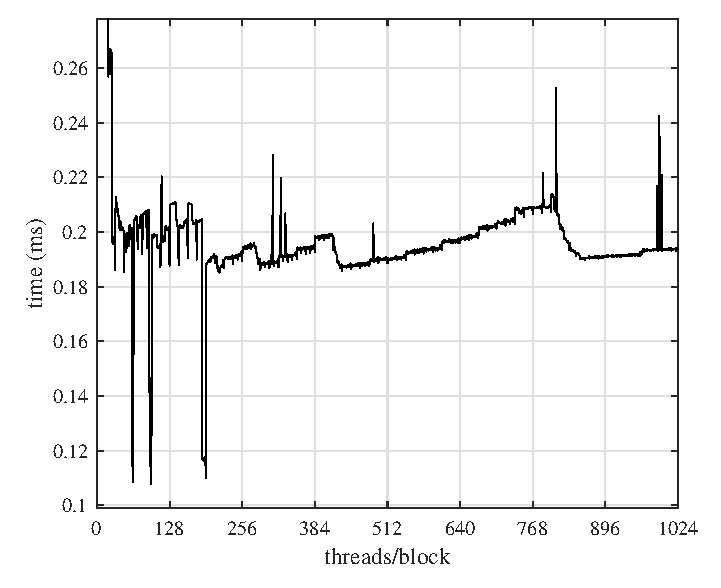
\includegraphics[width=5in]{figures/gpu_intro/ConvGPU_shared_12672_186taps.eps}
	\caption{Plot showing how execution time is affected by changing the number of threads per block.
	The optimal execution time for an example GPU kernel is $0.1078$ ms at the optimal $96$ threads per block.}
	\label{fig:ConvGPU_shared_12672_186taps}
\end{figure}
\begin{figure}
	\centering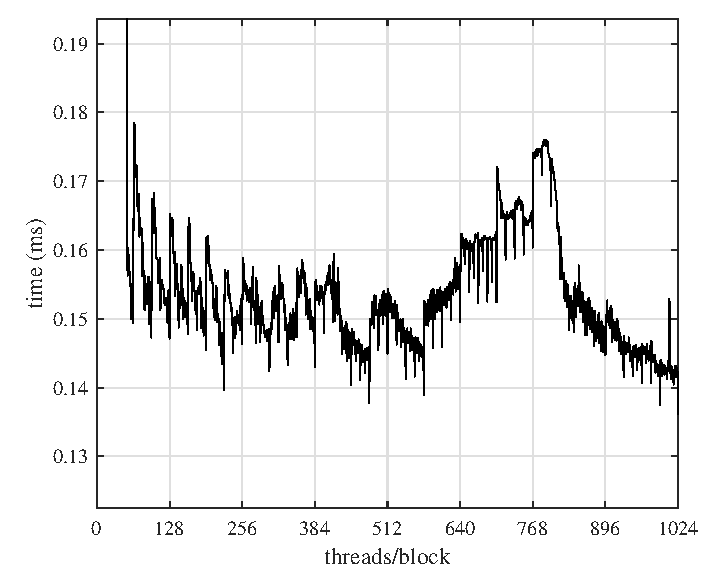
\includegraphics[width=5in]{figures/gpu_intro/ConvGPU_global_12672_186taps.eps}
	\caption{Plot showing the number of threads per block doesn't always drastically affect execution time.}
	\label{fig:ConvGPU_global_12672_186taps}
\end{figure}

While designing a custom GPU kernel to obtain a major speed up is satisfying,
CUDA has optimized GPU libraries that are extremely useful and efficient with exceptional documentation.
The CUDA libraries are written by NVIDIA engineers to maximize the performance of NVIDIA GPUs.
The libraries explained in this thesis include cuFFT, cuBLAS and cuSolverSp.

\subsection{CPU and GPU Pipelining}
While GPU kernels execute physically on the GPU, the GPU only executes instructions received from the host CPU.
The CPU is idle while it waits for GPU kernels to execute.
To introduce CPU and GPU pipelining, the CPU can be pipelined by performing other operations while waiting for the GPU to finish executing kernels.

A basic CPU GPU program with no pipelining is shown in Listing \ref{code:noPipe}.
The CPU acquires data from myADC on Line 5.
After the CPU takes time to acquire data, the data is copied from the host (CPU) to the device (GPU) on line 8.
The data is processed on the GPU once then the result is copied back to the device to host on line 9 and 10.
The cudaDeviceSynchronize function on line 13 blocks CPU until all GPU instructions are finished executing.
Note that the CPU is blocked during any host to device or device to host transfer.
Acquiring and copying data takes processing time on the CPU and GPU.
Figure \ref{fig:concurrentCPU_blocking} shows a block diagram of what is happening on the CPU and GPU in Listing \ref{code:noPipe} (end of the section).
The GPU is idle while the CPU is acquiring data and the CPU is idle while the GPU is processing.
\begin{figure}
	\centering\includegraphics[width=8.77in/100*55]{figures/gpu_intro/concurrentCPU_blocking.pdf}
	\caption{The typical approach of CPU and GPU operations. This block diagram shows the profile of Listing \ref{code:noPipe}.}
	\label{fig:concurrentCPU_blocking}
\end{figure}

Listing \ref{code:pipe} (end of the section) shows how to CPU and GPU operations can be pipelined.
Assuming data is already on the GPU from a prior computation, the CPU gives processing instructions to the GPU then acquires data.
The CPU then does an asynchronous data transfer to a temporary vector on the GPU.
The GPU first performs a device to device transfer from the temporary vector.
The GPU then runs the GPUkernel and transfers the result to the host.
Note that device to device transfers do not block the CPU.
This system suffers a full cycle latency.
\begin{figure}
	\centering\includegraphics[width=9.97in/100*55]{figures/gpu_intro/concurrentCPU_nonBlocking.pdf}
	\caption{GPU and CPU operations can be pipelined. This block diagram shows a profile of Listing \ref{code:pipe}.}
	\label{fig:concurrentCPU_nonBlocking}
\end{figure}

Pipelineing can be extended to multiple GPUs for even more throughput, but only suffer latency of copying memory to one GPU.
Figure \ref{fig:concurrentCPU_nonBlocking_multiGPU} shows a block diagram of how three GPUs can be pipelined.
A strong understanding of the full system is required to pipeline at this level.
\begin{figure}
	\centering\includegraphics[width=11.4in/100*55]{figures/gpu_intro/concurrentCPU_nonBlocking_multiGPU.pdf}
	\caption{A block diagram of pipelining a CPU with three GPUs.}
	\label{fig:concurrentCPU_nonBlocking_multiGPU}
\end{figure}

\singlespacing
\clearpage
\begin{lstlisting}[style=myCUDAstyle,caption={Example code Simple example of the CPU acquiring data from myADC, copying from host to device, processing data on the device then copying from device to host. No processing occurs on device while CPU is acquiring data.},label={code:noPipe}]
int main()
{
	...
	// CPU Acuire Data
	myADC.acquire(vec);
	
	// Launch instructions on GPU 
	cudaMemcpy(dev_vec0, vec,      numBytes, cudaMemcpyHostToDevice);
	GPUkernel<<<1, N>>>(dev_vec0);
	cudaMemcpy(vec,      dev_vec0, numBytes, cudaMemcpyDeviceToHost);
	
	// Synchronize CPU with GPU
	cudaDeviceSynchronize();
	...
}
\end{lstlisting}
\doublespacing
\singlespacing
\begin{lstlisting}[style=myCUDAstyle,caption={Example code Simple of the CPU acquiring data from myADC, copying from host to device, processing data on the device then copying from device to host. No processing occurs on device while CPU is acquiring data.},label={code:pipe}]
int main()
{
	...
	// Launch instructions on GPU 
	cudaMemcpy(dev_vec, dev_temp, numBytes, cudaMemcpyDeviceToDevice);
	GPUkernel<<<N, M>>>(dev_vec);
	cudaMemcpy(vec,     dev_vec,  numBytes, cudaMemcpyDeviceToHost);
	
	// CPU Acuire Data
	myADC.acquire(vec);
	cudaMemcpyAsync(dev_temp, vec, numBytes, cudaMemcpyHostToDevice);
	
	// Synchronize CPU with GPU
	cudaDeviceSynchronize();
	...
	
	...
	// Launch instructions on GPU 
	cudaMemcpy(dev_vec, dev_temp, numBytes, cudaMemcpyDeviceToDevice);
	GPUkernel<<<N, M>>>(dev_vec);
	cudaMemcpy(vec,     dev_vec,  numBytes, cudaMemcpyDeviceToHost);
	
	// CPU Acuire Data
	myADC.acquire(vec);
	cudaMemcpyAsync(dev_temp, vec, numBytes, cudaMemcpyHostToDevice);
	
	// Synchronize CPU with GPU
	cudaDeviceSynchronize();
	...
}
\end{lstlisting}
\doublespacing

\clearpage
\section{GPU Convolution}
\label{chap:gpu_convolution}
Convolution is one of the most important tools in digital signal processing.
The PAQ system explained uses convolution up to 26 times per packet, depending on the number of CMA iterations.
If convolution execution time can be reduced by 10 ms, the full system execution time can reduced by 260 ms.
This section will use the following notation: 
\begin{itemize}
\item The signal $\mathbf{x}$ is a vector of $N$ complex samples indexed by $x(n)$ where, $0 \leq \leq N-1$.
\item The filter $\mathbf{h}$ is a vector of $L$ complex samples indexed by $h(n)$ where, $0 \leq \leq L-1$.
\item The filtered signal $\mathbf{y}$ is a vector resulting from the convolution of $\mathbf{x}$ and $\mathbf{h}$. $\mathbf{y}$ is $C = N + L -1$ complex samples and is indexed by $y(n)$ where, $0 \leq n \leq C-1$.
\item The forward Fast Fourier Transform (FFT) of the vector $\mathbf{x}$ is denoted $\mathscr{F}(\mathbf{x})$.
\item The inverse Fast Fourier Transform (IFFT) of the vector $\mathbf{x}$ is denoted $\mathscr{F}^{-1}(\mathbf{x})$.
\end{itemize}

Discrete time convolution applies the filter $\mathbf{h}$ to the signal $\mathbf{x}$ resulting in the filter signal $\mathbf{y}$.
Convolution in the time domain is
\begin{equation}
y(n) = \sum^{L-1}_{m=0} x(m) h(n-m),
  \label{eq:simple_conv_time}
\end{equation}
and the frequency domain is
\begin{equation}
\mathbf{y} = \mathscr{F}^{-1}(\mathscr{F}(\mathbf{x})\times\mathscr{F}(\mathbf{h})).
  \label{eq:simple_conv_freq}
\end{equation}
Figure \ref{fig:freq_time_block} shows block diagrams for time-domain and frequency domain convolution.
\begin{figure}
	\centering\includegraphics[width=10.28in/100*55]{figures/gpu_convolution/convBlock.pdf}
	\caption{Block diagrams showing time-domain convolution and frequency-domain convolution.}
	\label{fig:freq_time_block}
\end{figure}
This section will show:
\begin{itemize}
\item GPU convolution is faster than CPU convolution with large data sets using execution time as a metric.
\item GPU convolution execution time is dependent more on memory access than floating point operations.
\item Performing batched GPU convolution invokes more parallelism and decreases execution time per batch.
\item Batched GPU frequency-domain convolution executes faster than batched GPU time-domain convolution.
\end{itemize}

\subsection{Floating Point Operation Comparison}
Traditionally the number of floating point operations (flops) is used to estimate how computationally intense an algorithm is. 
Each complex multiplication  
\begin{equation}
(A+jB)\times(C+jD) = (AC-BD)+j(AD+BC),
\end{equation}
requires $6$ flops, $4$ multiplications and $2$ additions/subtractions.
Output elements of $\mathbf{y}$ in Equation \eqref{eq:simple_conv_time} requires $8L = (6+2)L$ flops, $2$ extra flops are required for each summand.
The time-domain convolution requires
\begin{equation}
8LC \text{ flops},
\label{eq:flops_time_domain_conv}
\end{equation}
where $C=N+L-1$ is the length of the convolution result.

To leverage the Cooley-Tukey radix 2 Fast Fourier Transform (FFT) in frequency-domain convolution, common practice is to compute the $M$ point FFT where $M = 2^u$ and $u = {\left\lceil \log_2{\left(C\right)}  \right\rceil}$.
Both the CPU based Fastest Fourier Transform in the West (FFTW) library and the NVIDIA GPU cuFFT library use the Cooley-Tukey radix 2 FFT.
Each FFT or IFFT requires $5M\log_2(M)$ flops \cite{FFTW:2017,cooley1965algorithm}.
As shown by Equation \eqref{eq:simple_conv_freq}, frequency-domain convolution requires 
\begin{equation}
3\times5M\log_2(M)+6M \text{ flops},
\label{eq:flops_freq_domain_conv}
\end{equation}
from $3$ FFTs and $M$ point-to-point multiplications.

Sections \ref{sec:hardware} and \ref{sec:oqpsk_detector} show the PAQ system has one signal length, $N = \Lpkt = 12$,$672$ samples and two filter lengths $L = L_\text{df} = 23$ and $L = L_\text{eq} = 186$.
Figures \ref{fig:Theory186Tap_flops} through \ref{fig:Theory12672signal_flops} compare the number of flops required for time-domain and frequency-domain convolution.
The figures compare flops by fixing the signal length with variable filter length or visa versa.
These figures show applying a $186$ tap filter to a $12$,$672$ sample signal requires less flops in the frequency domain and
applying a $23$ tap filter to a $12$,$672$ sample signal requires less flops in the time domain.
\begin{figure}
	\centering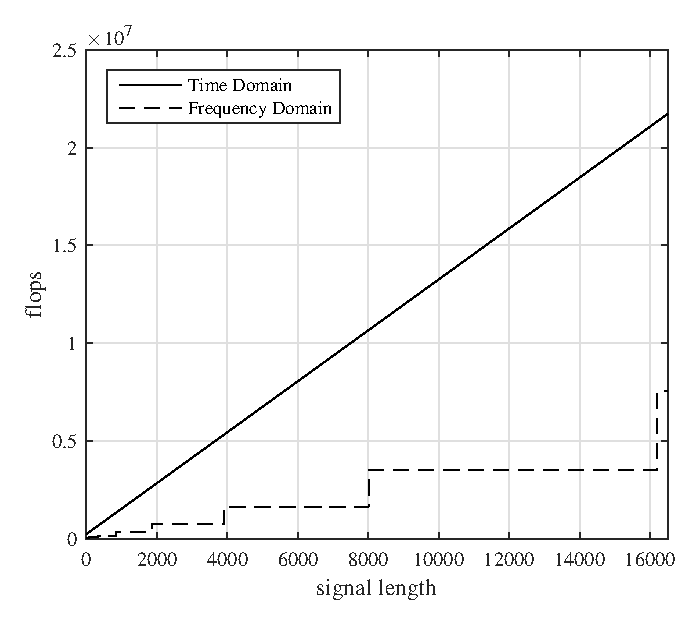
\includegraphics[width=5in]{figures/gpu_intro/Theory186Tap_flops.eps}
	\caption{Comparison of number of floating point operations (flops) required to convolve a variable length complex signal with a $186$ tap complex filter.}
	\label{fig:Theory186Tap_flops}
\end{figure}
\begin{figure}
	\centering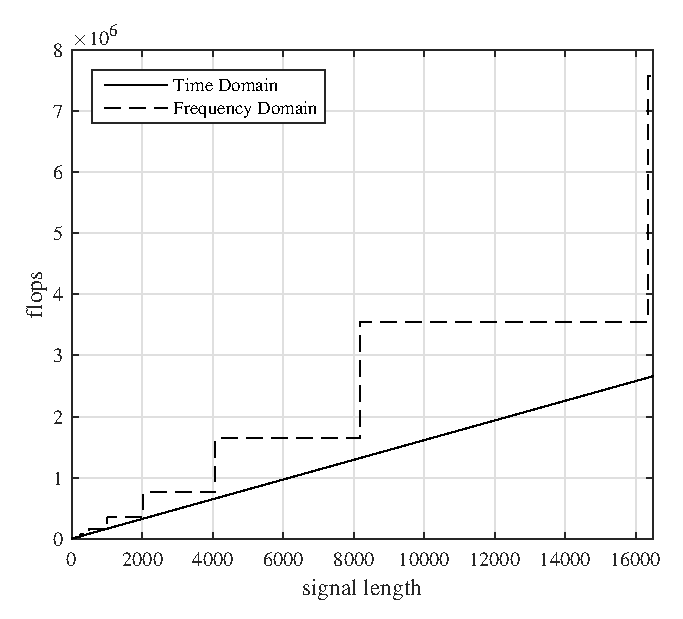
\includegraphics[width=5in]{figures/gpu_intro/Theory23Tap_flops.eps}
	\caption{Comparison of number of floating point operations (flops) required to convolve a variable length complex signal with a $23$ tap complex filter.}
	\label{fig:Theory23Tap_flops}
\end{figure}
\begin{figure} 
	\centering\includegraphics[width=5in]{figures/gpu_intro/Theory12672signal_flops.eps}
	\caption{Comparison of number of floating point operations (flops) required to convolve a $12$,$672$ sample complex signal with a variable length tap complex filter.}
	\label{fig:Theory12672signal_flops}
\end{figure}

\subsection{CPU and GPU Single Convolution Using Batch Processing Comparison}
\label{sec:cuda_convolution_single}
This section will show GPU convolution execution time is dependent more on memory access than the number of required floating point operations, while CPU convolution execution time is dependent on the number of floating point operations.
To illustrate these points, the execution time of the code in Listing \ref{code:convFun} (at the end of the chapter) was measured.
The code implements convolution five different ways:
\begin{itemize}
  \item time-domain convolution in a CPU,
  \item frequency-domain convolution in a CPU using the FFTW library,
  \item time-domain convolution in a GPU using global memory,
  \item time-domain convolution in a GPU using shared memory, and
  \item frequency-domain convolution in a GPU using the cuFFT library.
\end{itemize}

The three time-domain convolution implementations compute \eqref{eq:simple_conv_time} directly.
The two \newline frequency-domain convolution implementations compute \eqref{eq:simple_conv_freq}, using the CPU FFTW library and the GPU based cuFFT library.
The cuFFT library uses global memory and shared memory to be as fast and efficient as possible.
For a given signal and filter length, a good CUDA programmer can make an educated guess on which algorithm is faster.
There is no clear conclusion, until all the algorithms have been implemented and measured.

%The CPU implements Equation \eqref{eq:simple_conv_time} in ConvCPU directly on line $209$ using a function from lines $11$ to $34$.
%The CPU implements Equation \eqref{eq:simple_conv_freq} using the FFTW library on lines $214$ to $258$.
%
%The GPU implements time-domain convolution using global memory in lines $268$ to $277$.
%The GPU kernel ConvGPU on lines $36$ to $64$ is a parallel version of ConvCPU.
%ConvGPU performs time-domain convolution by fetching every element of the signal and filter from global memory.
%
%The GPU implements time-domain convolution using shared memory in lines $283$ to $292$.
%The GPU kernel ConvGPUshared on lines $67$ to $101$ is nearly identical to ConvGPU.
%Threads accessing the same elements of the filter in global memory can be a waste of valuable clock cycles.
%ConvGPUshared pays and initial price on lines $72$ to $76$ to move $L_\text{h}$ filter coefficients from off chip global memory to the on chip shared memory.
%Finally, the GPU implements frequency-domain convolution using the cuFFT library on lines $298$ to $326$.
%
%The questions are:
%Do flops have a direct relationship to execution time on CPUs? 
%Do flops have a direct relationship to execution time on GPUs? 
%When is the initial cost to use shared memory worth it?
%When should convolution be done in the frequency domain?
%
%The short answer to all of the questions is: GPU execution time depend on the signal length, filter length, CPU, GPU and memory.
%A good CUDA programmer can make an educated guess on which algorithm may be faster in the GPU, but until all the algorithms have been implemented and timed, there is no definite answer.

All the memory transfers to and from the GPU were timed for a fair comparison of GPU to CPU execution time.
Table \ref{tab:CPUvsGPUtimingTable} shows how the execution time was measured for each convolution implementation.
\begin{table}
\caption{Defining start and stop lines for timing comparison in Listing \ref{code:convFun}.}
\begin{center}
\begin{tabular}{llll}
	\toprule
	Algorithm 				& Function		& Start Line	& Stop  Line		\\ \midrule
	CPU time domain 		& ConvCPU 		& 208			& 210 				\\
	CPU frequency domain 	& FFTW 			& 213			& 259 				\\
	GPU time domain global 	& ConvGPU 		& 267			& 278				\\
	GPU time domain shared 	& ConvGPUshared & 282			& 293				\\
	GPU frequency domain 	& cuFFT			& 301			& 327				\\ 
	\bottomrule
\end{tabular}
\end{center}
\label{tab:CPUvsGPUtimingTable}
\end{table}
Figures \ref{fig:CPUvsGPU_1batch_186taps_varySignal_noMin} through \ref{fig:CPUvsGPU_1batch_12672signal_varyFilter} compare execution time of the five different convolution implementations by fixing the filter length with variable signal length or vise versa.
Sub-windows emphasize points that are of interest to the PAQ system.
The variations in the time-domain CPU execution times are due to the claims on the host CPU resources by the operating system.
To clean up the time samples, local minima were found in windows ranging from 3 to 15 samples.
The smallest windows possible were used to produce the results.
\begin{figure}
	\centering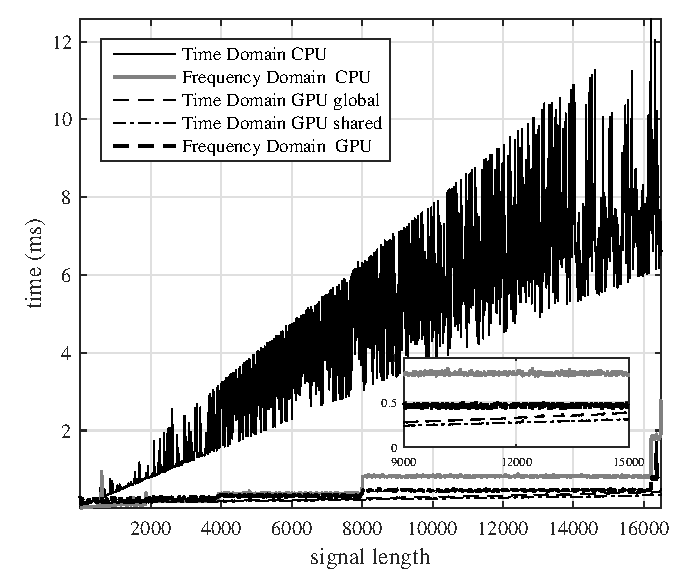
\includegraphics[width=5in]{figures/gpu_intro/CPUvsGPU_1batch_186taps_varySignal_noMin.eps}
	\caption{Comparison of a complex convolution on CPU and GPU. The signal length is variable and the filter is fixed at $186$ taps. The comparison is messy without lower bounding.}
	\label{fig:CPUvsGPU_1batch_186taps_varySignal_noMin}
\end{figure}
\begin{figure}
	\centering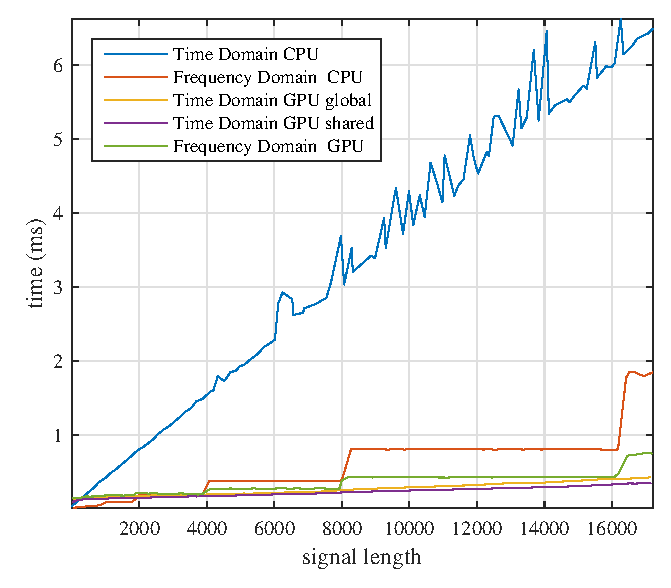
\includegraphics[width=5in]{figures/gpu_intro/CPUvsGPU_1batch_186taps_varySignal.eps}
	\caption{Comparison of a complex convolution on CPU and GPU. The signal length is variable and the filter is fixed at $186$ taps. A lower bound was applied by searching for a local minima in 15 sample width windows.}
	\label{fig:CPUvsGPU_1batch_186taps_varySignal}
\end{figure}
\begin{figure}
	\centering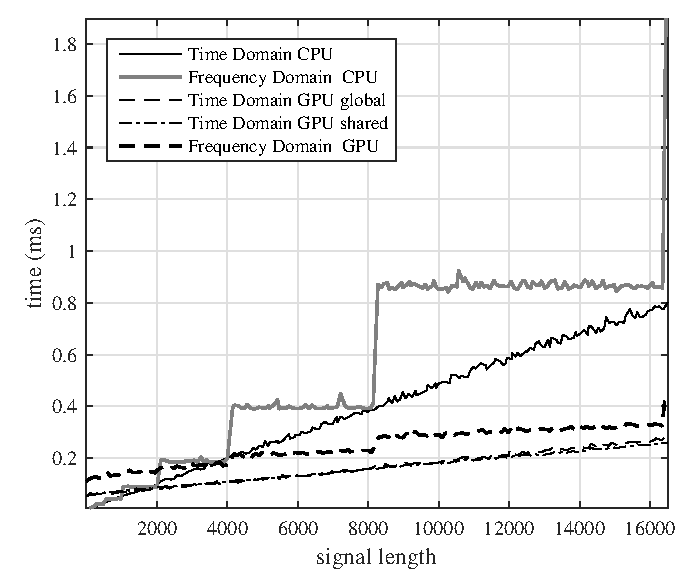
\includegraphics[width=5in]{figures/gpu_intro/CPUvsGPU_1batch_23taps_varySignal.eps}
	\caption{Comparison of a complex convolution on CPU and GPU. The signal length is variable and the filter is fixed at $23$ taps. A lower bound was applied by searching for a local minima in 5 sample width windows.}
	\label{fig:CPUvsGPU_1batch_23taps_varySignal}
\end{figure}
\begin{figure}
	\centering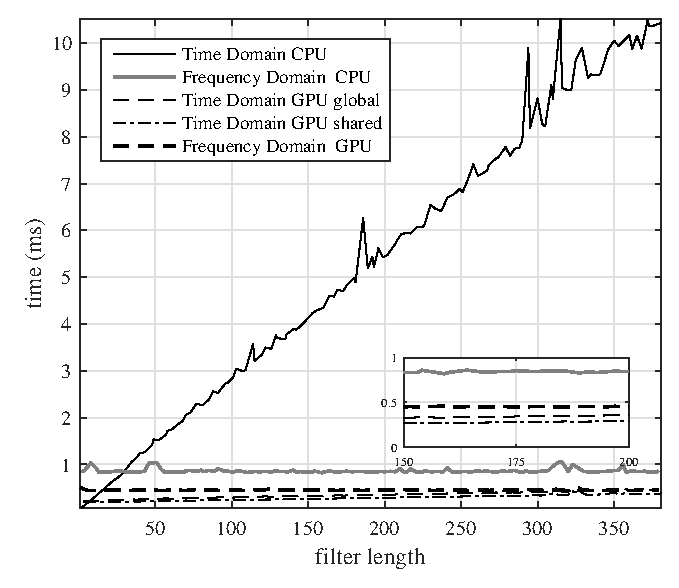
\includegraphics[width=5in]{figures/gpu_intro/CPUvsGPU_1batch_12672signal_varyFilter.eps}
	\caption{Comparison of a complex convolution on CPU and GPU. The filter length is variable and the signal is fixed at $12$,$672$ samples. A lower bound was applied by searching for a local minima in three sample width windows.}
	\label{fig:CPUvsGPU_1batch_12672signal_varyFilter}
\end{figure}

Comparing Figures \ref{fig:CPUvsGPU_1batch_186taps_varySignal} through \ref{fig:CPUvsGPU_1batch_12672signal_varyFilter}
to Figures \ref{fig:Theory186Tap_flops} through
\ref{fig:Theory12672signal_flops} 
shows
CPU and GPU convolution have the same structure that the number of flops predicted, except GPU convolution is not affected as much by varied signal or filter lengths.
The convolution execution time comparison demonstrates the observation that most GPU kernels execution time is limited by memory bandwidth not computational resources.
Tables \ref{tab:CPUvsGPUtable_12672_186} and \ref{tab:CPUvsGPUtable_12672_23} show the GPU time-domain algorithm using shared memory is fastest for the signal length and filter lengths of the PAQ system, when performing a single complex convolution.
\begin{table}
\caption{Convolution computation times with signal length $12$,$672$ and filter length $186$ on a Tesla K40c GPU.}
\begin{center}
\begin{tabular}{lll}
	\toprule
	Algorithm 				& Function or Library		& Execution Time (ms) \\ \midrule
	CPU time domain 		& ConvCPU 					& 6.2683		\\
	CPU frequency domain 	& FFTW 						& 0.8519		\\
	GPU time domain global 	& ConvGPU 					& 0.3467		\\
	GPU time domain shared 	& ConvGPUshared 			& 0.2857		\\
	GPU frequency domain 	& cuFFT						& 0.4490		\\ 
	\bottomrule
\end{tabular}
\end{center}
\label{tab:CPUvsGPUtable_12672_186}
\end{table}
\begin{table}
\caption{Convolution computation times with signal length $12$,$672$ and filter length $23$ on a Tesla K40c GPU.}
\begin{center}
\begin{tabular}{lll}
	\toprule
	Algorithm 				& Function or Library		& Execution Time (ms) \\ \midrule
%	CPU time domain 		& ConvCPU 					& 0.5878		\\
%	CPU frequency domain 	& FFTW 						& 0.8417		\\
%	GPU time domain global 	& ConvGPU 					& 0.4476		\\
%	GPU time domain shared 	& ConvGPUshared 			& 0.1971		\\
%	GPU frequency domain 	& cuFFT						& 0.3360		\\
	CPU time domain 		& ConvCPU 					& 0.6429		\\
	CPU frequency domain 	& FFTW 						& 0.8899		\\
	GPU time domain global 	& ConvGPU 					& 0.2406		\\
	GPU time domain shared 	& ConvGPUshared 			& 0.2346		\\
	GPU frequency domain 	& cuFFT						& 0.3231		\\
	\bottomrule
\end{tabular}
\end{center}
\label{tab:CPUvsGPUtable_12672_23}
\end{table}

\subsection{Convolution Using Batch Processing}
\label{sec:batched_convolution}
Section \ref{sec:cuda_convolution_single}, illustrated convolving one signal with one filter, does not leverage the full power of parallel processing in GPUs.
The received signal in the PAQ system has a packetized structure with $3104$ packets per $1907$ ms.
Rather than processing each packet separately, the packets may be buffered and processed in a batch.
Batch processing in GPUs has less CPU overhead and introduces an extra level of parallelism.
Batch processing has faster execution time per packet, than processing packets separately.
CUDA has many libraries that have batch processing, including cuFFT, cuBLAS and cuSolverSp.
Haidar et al. \cite{haidar2015optimization} showed batched libraries achieve more Gflops, than calling GPU kernels multiple times.
Listing \ref{code:batchedConvFun} (at the end of the chapter) shows three GPU implementations of convolution using batch processing and Table \ref{tab:BatchedGPUtimingTable} shows how the execution time of the code was measured.
\begin{table}
\caption{Defining start and stop lines for execution time comparison in Listing \ref{code:batchedConvFun}.}
\begin{center}
\begin{tabular}{llll}
	\toprule
	Algorithm 				& Function		& Start Line	& Stop  Line		\\ \midrule
	GPU time domain global 	& ConvGPU 		& 197			& 204				\\
	GPU time domain shared 	& ConvGPUshared & 212			& 219				\\
	GPU frequency domain 	& cuFFT			& 227			& 245				\\ 
	\bottomrule
\end{tabular}
\end{center}
\label{tab:BatchedGPUtimingTable}
\end{table}

Figure \ref{fig:CPUvsGPU_varyBatches_186taps_12672signal} compares execution time of convolution using batch processing as the number of packets increases, note that no lower bounding was used.
This figure shows that frequency-domain convolution leverages batch processing better than time-domain convolution.
As expected, CPU-based convolution using batch processing is not competitive with GPU-based convolution using batch processing and thus CPU-batched processing is not explored any further.
\begin{figure}
	\centering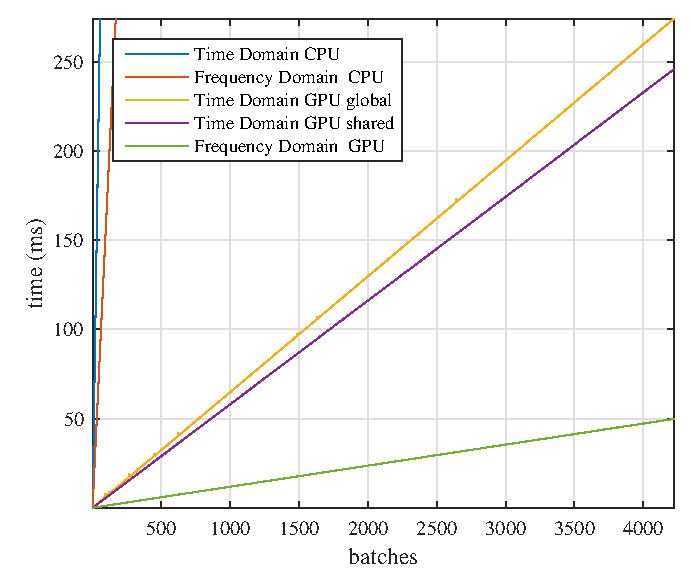
\includegraphics[width=5in]{figures/gpu_intro/CPUvsGPU_varyBatches_186taps_12672signal.eps}
	\caption{Comparison of a batched complex convolution on a CPU and GPU. The number of batches is variable while the signal and filter length is set to $12$,$672$ and $186$.}
	\label{fig:CPUvsGPU_varyBatches_186taps_12672signal}
\end{figure}

Now that the GPU and CPU execution time is not being compared, Table \ref{tab:BatchedGPUtimingTable} shows execution times include only GPU kernels and exclude memory transfers.
Figure \ref{fig:CPUvsGPU_varyBatches_186taps_12672signal_timePerBatch} compares GPU convolution using batch processing execution time per batch as the number of packets increases.
The figure shows execution time per batch decreases as the number of packets increases but stops improving after 70 packets.
\begin{figure}
	\centering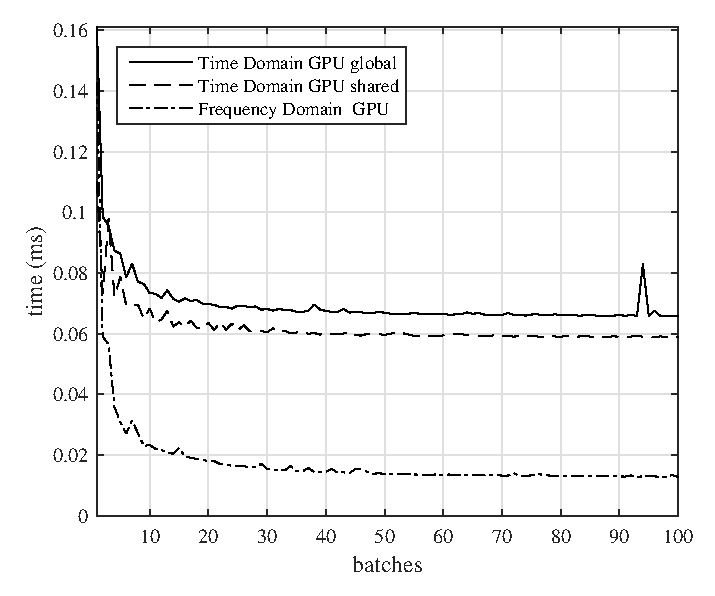
\includegraphics[width=5in]{figures/gpu_intro/CPUvsGPU_varyBatches_186taps_12672signal_timePerBatch.eps}
	\caption{Comparison on execution time per batch for complex convolution. The number of batches is variable while the signal and filter length is set to $12$,$672$ and $186$.}
	\label{fig:CPUvsGPU_varyBatches_186taps_12672signal_timePerBatch}
\end{figure}


Figures \ref{fig:CPUvsGPU_3104batch_186taps_varySignal} through \ref{fig:CPUvsGPU_3104batch_12672signal_varyFilter} 
compare execution time of the three GPU convolution implementations by fixing the filter length with variable signal length or vise versa.
Tables \ref{tab:Batched_CPUvsGPUtable_12672_186} and \ref{tab:Batched_CPUvsGPUtable_12672_23} 
show the execution times for the signal length and filter lengths of the PAQ system when performing convolution using batch processing.
Frequency-domain convolution using batch processing is fastest for $186$ tap filters while 
time-domain convolution using batch processing and shared memory is fastest for $23$ tap filters.
\begin{figure}
	\centering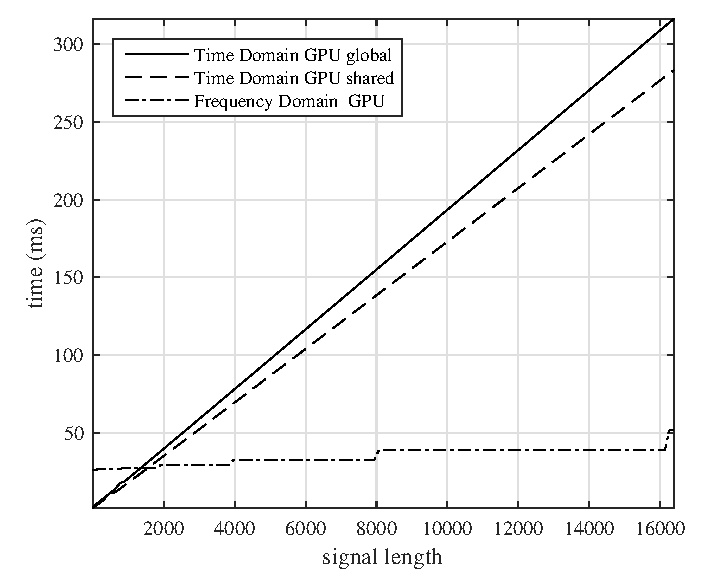
\includegraphics[width=5in]{figures/gpu_intro/CPUvsGPU_3104batch_186taps_varySignal.eps}
	\caption{Comparison of complex convolution using batch processing on a GPU. The signal length is variable and the filter is fixed at $186$ taps.}
	\label{fig:CPUvsGPU_3104batch_186taps_varySignal}
\end{figure}
\begin{figure}
	\centering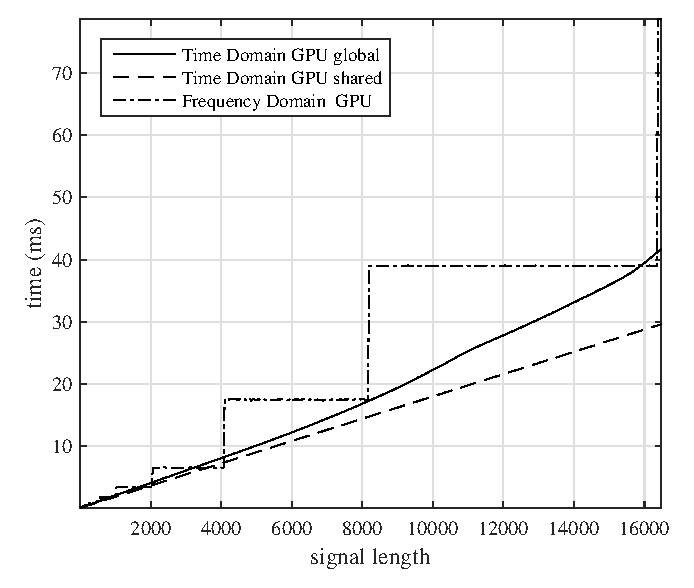
\includegraphics[width=5in]{figures/gpu_intro/CPUvsGPU_3104batch_23taps_varySignal.eps}
	\caption{Comparison of complex convolution using batch processing on a GPU. The signal length is variable and the filter is fixed at $23$ taps.}
	\label{fig:CPUvsGPU_3104batch_23taps_varySignal}
\end{figure}
\begin{figure}
	\centering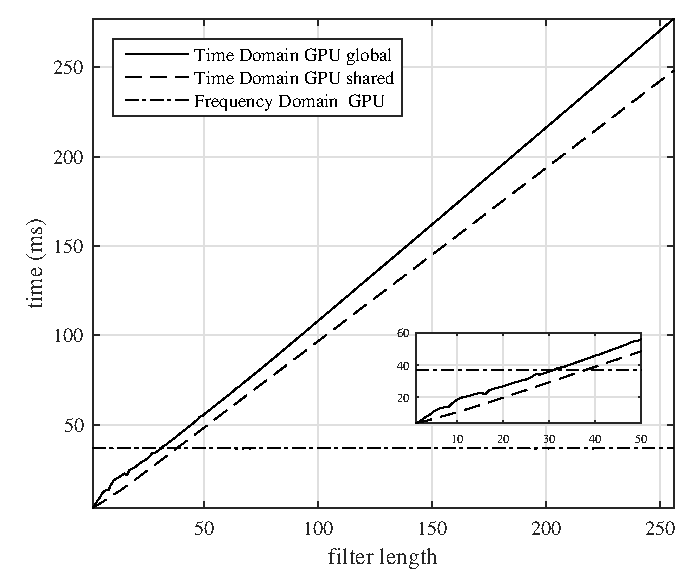
\includegraphics[width=5in]{figures/gpu_intro/CPUvsGPU_3104batch_12672signal_varyFilter.eps}
	\caption{Comparison of complex convolution using batch processing on a GPU. The filter length is variable and the signal length is set to $12$,$672$ samples.}
	\label{fig:CPUvsGPU_3104batch_12672signal_varyFilter}
\end{figure}
\begin{table}
\caption{Convolution using batch processing execution times with for a $12$,$672$ sample signal and $186$ tap filter on a Tesla K40c GPU.}
\begin{center}
\begin{tabular}{lll}
	\toprule
	Algorithm 				& Function or Library		& Execution Time (ms) \\ \midrule
	GPU time domain global 	& ConvGPU 					& 201.3		\\
	GPU time domain shared 	& ConvGPUshared 			& 180.3		\\
	GPU frequency domain 	& cuFFT						& 36.8 		\\ 
	\bottomrule
\end{tabular}
\end{center}
\label{tab:Batched_CPUvsGPUtable_12672_186}
\end{table}
\begin{table}
\caption{Convolution using batch processing execution times with for a $12$,$672$ sample signal and $23$ tap filter on a Tesla K40c GPU.}
\begin{center}
\begin{tabular}{lll}
	\toprule
	Algorithm 				& Function or Library		& Execution Time (ms) \\ \midrule
	GPU time domain global 	& ConvGPU 					& 29.5		\\
	GPU time domain shared 	& ConvGPUshared 			& 22.7			\\
	GPU frequency domain 	& cuFFT						& 39.0		\\ 
	\bottomrule
\end{tabular}
\end{center}
\label{tab:Batched_CPUvsGPUtable_12672_23}
\end{table}

Until now, convolving one signal with only one filter has been considered.
Figure \ref{fig:thisThesisBlock} showed the received signal is filtered by two cascaded filters: 
an equalizer filter and a detection filter.
The block diagrams in Figure \ref{fig:freq_time_block_cascade} show the steps required for cascading time-domain and frequency-domain convolution.

Comparing the block diagrams in Figures \ref{fig:freq_time_block_cascade} and \ref{fig:freq_time_block}, cascading two filters in the frequency domain only requires an extra FFT and point-by-point complex multiplication, while cascading filters in the time domain requires two time-domain convolutions.
The first time-domain convolution produces a composite filter from the convolution of the $186$ sample equalizer filter with the $23$ tap detection filter.
The second time-domain convolution applies the composite $208 = 186 + 23 - 1$ tap filter to a $12$,$672$ sample signal.
Table \ref{tab:Batched_CPUvsGPUtable_12672_23_186} shows the execution times for the signal length and filter lengths of the PAQ system, when performing cascaded convolution using batch processing.
Cascaded-convolution using batch processing in the frequency domain is fastest.
\begin{figure}
	\centering\includegraphics[width=10.28in/100*55]{figures/gpu_convolution/CascadeConvBlock.pdf}
	\caption{Block diagrams showing showing cascaded time-domain convolution and frequency-domain convolution.}
	\label{fig:freq_time_block_cascade}
\end{figure}
\begin{table}
\caption{Batched convolution execution times with for a $12$,$672$ sample signal and cascaded $23$ and $186$ tap filter on a Tesla K40c GPU.}
\begin{center}
\begin{tabular}{lll}
	\toprule
	Algorithm 				& Function or Library		& Execution Time (ms) \\ \midrule
	GPU time domain global 	& ConvGPU 					& 228.8		\\
	GPU time domain shared 	& ConvGPUshared 			& 205.0		\\
	GPU frequency domain 	& cuFFT						& 39.0		\\ 
	\bottomrule
\end{tabular}
\end{center}
\label{tab:Batched_CPUvsGPUtable_12672_23_186}
\end{table}



\singlespacing
\clearpage
\begin{lstlisting}[style=myCUDAstyle,language=C++,caption={CUDA code to performing complex convolution five different ways: time domain CPU, frequency domain CPU time domain GPU, time domain GPU using shared memory and frequency domain GPU.},label={code:convFun}]
#include <iostream>
#include <stdlib.h>
#include <math.h>
#include <cufft.h>
#include <fstream>
#include <string>
#include <fftw3.h>
using namespace std;


void ConvCPU(cufftComplex* y,cufftComplex* x,cufftComplex* h,int Lx,int Lh){
	for(int yIdx = 0; yIdx < Lx+Lh-1; yIdx++){
		cufftComplex temp;
		temp.x = 0;
		temp.y = 0;
		for(int hIdx = 0; hIdx < Lh; hIdx++){
			int xAccessIdx = yIdx-hIdx;
			if(xAccessIdx>=0 && xAccessIdx<Lx){
				// temp += x[xAccessIdx]*h[hIdx];
				float A = x[xAccessIdx].x;
				float B = x[xAccessIdx].y;
				float C = h[hIdx].x;
				float D = h[hIdx].y;
				cufftComplex result;
				result.x = A*C-B*D;
				result.y = A*D+B*C;
				temp.x += result.x;
				temp.y += result.y;
			}
		}
		y[yIdx] = temp;
	}

}

__global__ void ConvGPU(cufftComplex* y,cufftComplex* x,cufftComplex* h,int Lx,int Lh){
	int yIdx = blockIdx.x*blockDim.x + threadIdx.x;

	int lastThread = Lx+Lh-1;

	// don't access elements out of bounds
	if(yIdx >= lastThread)
		return;

	cufftComplex temp;
	temp.x = 0;
	temp.y = 0;
	for(int hIdx = 0; hIdx < Lh; hIdx++){
		int xAccessIdx = yIdx-hIdx;
		if(xAccessIdx>=0 && xAccessIdx<Lx){
			// temp += x[xAccessIdx]*h[hIdx];
			float A = x[xAccessIdx].x;
			float B = x[xAccessIdx].y;
			float C = h[hIdx].x;
			float D = h[hIdx].y;
			cufftComplex result;
			result.x = A*C-B*D;
			result.y = A*D+B*C;
			temp.x += result.x;
			temp.y += result.y;
		}
	}
	y[yIdx] = temp;
}


__global__ void ConvGPUshared(cufftComplex* y,cufftComplex* x,cufftComplex* h,int Lx,int Lh){
	int yIdx = blockIdx.x*blockDim.x + threadIdx.x;

	int lastThread = Lx+Lh-1;

	extern __shared__ cufftComplex h_shared[];
	if(threadIdx.x < Lh){
		h_shared[threadIdx.x] = h[threadIdx.x];
	}
	__syncthreads();

	// don't access elements out of bounds
	if(yIdx >= lastThread)
		return;

	cufftComplex temp;
	temp.x = 0;
	temp.y = 0;
	for(int hIdx = 0; hIdx < Lh; hIdx++){
		int xAccessIdx = yIdx-hIdx;
		if(xAccessIdx>=0 && xAccessIdx<Lx){
			// temp += x[xAccessIdx]*h[hIdx];
			float A = x[xAccessIdx].x;
			float B = x[xAccessIdx].y;
			float C = h_shared[hIdx].x;
			float D = h_shared[hIdx].y;
			cufftComplex result;
			result.x = A*C-B*D;
			result.y = A*D+B*C;
			temp.x += result.x;
			temp.y += result.y;
		}
	}
	y[yIdx] = temp;
}

__global__ void PointToPointMultiply(cufftComplex* v0, cufftComplex* v1, int lastThread){
	int i = blockIdx.x*blockDim.x + threadIdx.x;

	// don't access elements out of bounds
	if(i >= lastThread)
		return;
	float A = v0[i].x;
	float B = v0[i].y;
	float C = v1[i].x;
	float D = v1[i].y;

	// (A+jB)(C+jD) = (AC-BD) + j(AD+BC)
	cufftComplex result;
	result.x = A*C-B*D;
	result.y = A*D+B*C;

	v0[i] = result;
}

__global__ void ScalarMultiply(cufftComplex* vec0, float scalar, int lastThread){
	int i = blockIdx.x*blockDim.x + threadIdx.x;

	// Don't access elements out of bounds
	if(i >= lastThread)
		return;
	cufftComplex scalarMult;
	scalarMult.x = vec0[i].x*scalar;
	scalarMult.y = vec0[i].y*scalar;
	vec0[i] = scalarMult;
}

int main(){
	int N = 1000;
	int L = 186;
	int C = N + L - 1;
	int M = pow(2, ceil(log(C)/log(2)));

	cufftComplex *mySignal1;
	cufftComplex *mySignal2;
	cufftComplex *mySignal2_fft;

	cufftComplex *myFilter1;
	cufftComplex *myFilter2;
	cufftComplex *myFilter2_fft;

	cufftComplex *myConv1;
	cufftComplex *myConv2;
	cufftComplex *myConv2_timeReversed;
	cufftComplex *myConv3;
	cufftComplex *myConv4;
	cufftComplex *myConv5;

	mySignal1      		= (cufftComplex*)malloc(N*sizeof(cufftComplex));
	mySignal2      		= (cufftComplex*)malloc(M*sizeof(cufftComplex));
	mySignal2_fft  		= (cufftComplex*)malloc(M*sizeof(cufftComplex));

	myFilter1      		= (cufftComplex*)malloc(L*sizeof(cufftComplex));
	myFilter2      		= (cufftComplex*)malloc(M*sizeof(cufftComplex));
	myFilter2_fft  		= (cufftComplex*)malloc(M*sizeof(cufftComplex));

	myConv1        		= (cufftComplex*)malloc(C*sizeof(cufftComplex));
	myConv2        		= (cufftComplex*)malloc(M*sizeof(cufftComplex));
	myConv2_timeReversed= (cufftComplex*)malloc(M*sizeof(cufftComplex));
	myConv3        		= (cufftComplex*)malloc(C*sizeof(cufftComplex));
	myConv4        		= (cufftComplex*)malloc(C*sizeof(cufftComplex));
	myConv5        		= (cufftComplex*)malloc(M*sizeof(cufftComplex));

	srand(time(0));
	for(int i = 0; i < N; i++){
		mySignal1[i].x = rand()%100-50;
		mySignal1[i].y = rand()%100-50;
	}

	for(int i = 0; i < L; i++){
		myFilter1[i].x = rand()%100-50;
		myFilter1[i].y = rand()%100-50;
	}

	cufftComplex *dev_mySignal3;
	cufftComplex *dev_mySignal4;
	cufftComplex *dev_mySignal5;

	cufftComplex *dev_myFilter3;
	cufftComplex *dev_myFilter4;
	cufftComplex *dev_myFilter5;

	cufftComplex *dev_myConv3;
	cufftComplex *dev_myConv4;
	cufftComplex *dev_myConv5;

	cudaMalloc(&dev_mySignal3, N*sizeof(cufftComplex));
	cudaMalloc(&dev_mySignal4, N*sizeof(cufftComplex));
	cudaMalloc(&dev_mySignal5, M*sizeof(cufftComplex));

	cudaMalloc(&dev_myFilter3, L*sizeof(cufftComplex));
	cudaMalloc(&dev_myFilter4, L*sizeof(cufftComplex));
	cudaMalloc(&dev_myFilter5, M*sizeof(cufftComplex));

	cudaMalloc(&dev_myConv3,   C*sizeof(cufftComplex));
	cudaMalloc(&dev_myConv4,   C*sizeof(cufftComplex));
	cudaMalloc(&dev_myConv5,   M*sizeof(cufftComplex));


	/**
	 * Time-domain Convolution CPU
	 */
	ConvCPU(myConv1,mySignal1,myFilter1,N,L);

	/**
	 * Frequency Domain Convolution CPU
	 */
	fftwf_plan forwardPlanSignal = fftwf_plan_dft_1d(M, (fftwf_complex*)mySignal2,    (fftwf_complex*)mySignal2_fft, 	   FFTW_FORWARD, FFTW_MEASURE);
	fftwf_plan forwardPlanFilter = fftwf_plan_dft_1d(M, (fftwf_complex*)myFilter2, 	 (fftwf_complex*)myFilter2_fft, 	   FFTW_FORWARD, FFTW_MEASURE);
	fftwf_plan backwardPlanConv  = fftwf_plan_dft_1d(M, (fftwf_complex*)mySignal2_fft,(fftwf_complex*)myConv2_timeReversed, FFTW_FORWARD, FFTW_MEASURE);

	cufftComplex zero; zero.x = 0; zero.y = 0;
	for(int i = 0; i < M; i++){
		if(i<N)
			mySignal2[i] = mySignal1[i];
		else
			mySignal2[i] = zero;

		if(i<L)
			myFilter2[i] = myFilter1[i];
		else
			myFilter2[i] = zero;
	}

	fftwf_execute(forwardPlanSignal);
	fftwf_execute(forwardPlanFilter);

	for (int i = 0; i < M; i++){
		// mySignal2_fft = mySignal2_fft*myFilter2_fft;
		float A = mySignal2_fft[i].x;
		float B = mySignal2_fft[i].y;
		float C = myFilter2_fft[i].x;
		float D = myFilter2_fft[i].y;
		cufftComplex result;
		result.x = A*C-B*D;
		result.y = A*D+B*C;
		mySignal2_fft[i] = result;
	}

	fftwf_execute(backwardPlanConv);

	// myConv2 from fftwf must be time reversed and scaled
	// to match Matlab, myConv1, myConv3, myConv4 and myConv5
	cufftComplex result;
	for (int i = 0; i < M; i++){
		result.x = myConv2_timeReversed[M-i].x/M;
		result.y = myConv2_timeReversed[M-i].y/M;
		myConv2[i] = result;
	}
	result.x = myConv2_timeReversed[0].x/M;
	result.y = myConv2_timeReversed[0].y/M;
	myConv2[0] = result;

	fftwf_destroy_plan(forwardPlanSignal);
	fftwf_destroy_plan(forwardPlanFilter);
	fftwf_destroy_plan(backwardPlanConv);


	/**
	 * Time-domain Convolution GPU Using Global Memory
	 */
	cudaMemcpy(dev_mySignal3, mySignal1, sizeof(cufftComplex)*N, cudaMemcpyHostToDevice);
	cudaMemcpy(dev_myFilter3, myFilter1, sizeof(cufftComplex)*L, cudaMemcpyHostToDevice);

	int T_B = 512;
	int B = C/T_B;
	if(C % T_B > 0)
		B++;
	ConvGPU<<<B, T_B>>>(dev_myConv3, dev_mySignal3, dev_myFilter3, N, L);

	cudaMemcpy(myConv3, dev_myConv3, C*sizeof(cufftComplex), cudaMemcpyDeviceToHost);


	/**
	 * Time-domain Convolution GPU Using Shared Memory
	 */
	cudaMemcpy(dev_mySignal4, mySignal1, sizeof(cufftComplex)*N, cudaMemcpyHostToDevice);
	cudaMemcpy(dev_myFilter4, myFilter1, sizeof(cufftComplex)*L, cudaMemcpyHostToDevice);

	T_B = 512;
	B = C/T_B;
	if(C % T_B > 0)
		B++;
	ConvGPUshared<<<B, T_B,L*sizeof(cufftComplex)>>>(dev_myConv4, dev_mySignal4, dev_myFilter4, N, L);

	cudaMemcpy(myConv4, dev_myConv4, C*sizeof(cufftComplex), cudaMemcpyDeviceToHost);


	/**
	 * Frequency-domain Convolution GPU
	 */
	cufftHandle plan;
	int n[1] = {M};
	cufftPlanMany(&plan,1,n,NULL,1,1,NULL,1,1,CUFFT_C2C,1);

	cudaMemset(dev_mySignal5, 0, 	     M*sizeof(cufftComplex));
	cudaMemset(dev_myFilter5, 0, 	     M*sizeof(cufftComplex));

	cudaMemcpy(dev_mySignal5, mySignal2, M*sizeof(cufftComplex), cudaMemcpyHostToDevice);
	cudaMemcpy(dev_myFilter5, myFilter2, M*sizeof(cufftComplex), cudaMemcpyHostToDevice);

	cufftExecC2C(plan, dev_mySignal5, dev_mySignal5, CUFFT_FORWARD);
	cufftExecC2C(plan, dev_myFilter5, dev_myFilter5, CUFFT_FORWARD);

	T_B = 512;
	B = M/T_B;
	if(M % T_B > 0)
		B++;
	PointToPointMultiply<<<B, T_B>>>(dev_mySignal5, dev_myFilter5, M);

	cufftExecC2C(plan, dev_mySignal5, dev_mySignal5, CUFFT_INVERSE);

	T_B = 128;
	B = M/T_B;
	if(M % T_B > 0)
		B++;
	float scalar = 1.0/((float)M);
	ScalarMultiply<<<B, T_B>>>(dev_mySignal5, scalar, M);

	cudaMemcpy(myConv5, dev_mySignal5, M*sizeof(cufftComplex), cudaMemcpyDeviceToHost);

	cufftDestroy(plan);

	free(mySignal1);
	free(mySignal2);

	free(myFilter1);
	free(myFilter2);

	free(myConv1);
	free(myConv2);
	free(myConv2_timeReversed);
	free(myConv3);
	free(myConv4);
	free(myConv5);
	fftwf_cleanup();

	cudaFree(dev_mySignal3);
	cudaFree(dev_mySignal4);
	cudaFree(dev_mySignal5);

	cudaFree(dev_myFilter3);
	cudaFree(dev_myFilter4);
	cudaFree(dev_myFilter5);

	cudaFree(dev_myConv3);
	cudaFree(dev_myConv4);
	cudaFree(dev_myConv5);

	return 0;
}
\end{lstlisting}
\doublespacing

\singlespacing
\clearpage
\begin{lstlisting}[style=myCUDAstyle,language=C++,caption={CUDA code to perform batched complex convolution three different ways in a GPU: time domain using global memory, time domain using shared memory and frequency domain GPU.},label={code:batchedConvFun}]
#include <cufft.h>
#include <iostream>
using namespace std;

__global__ void ConvGPU(cufftComplex* y_out,cufftComplex* x_in,cufftComplex* h_in,int Lx,int Lh,int maxThreads){
	int threadNum = blockIdx.x*blockDim.x + threadIdx.x;
	int convLength = Lx+Lh-1;

	// Don't access elements out of bounds
	if(threadNum >= maxThreads)
		return;

	int batch = threadNum/convLength;
	int yIdx  = threadNum%convLength;
	cufftComplex* x = &x_in[Lx*batch];
	cufftComplex* h = &h_in[Lh*batch];
	cufftComplex* y = &y_out[convLength*batch];

	cufftComplex temp;
	temp.x = 0;
	temp.y = 0;
	for(int hIdx = 0; hIdx < Lh; hIdx++){
		int xAccessIdx = yIdx-hIdx;
		if(xAccessIdx>=0 && xAccessIdx<Lx){
			// temp += x[xAccessIdx]*h[hIdx];
			// (A+jB)(C+jD) = (AC-BD) + j(AD+BC)
			float A = x[xAccessIdx].x;
			float B = x[xAccessIdx].y;
			float C = h[hIdx].x;
			float D = h[hIdx].y;
			cufftComplex complexMult;
			complexMult.x = A*C-B*D;
			complexMult.y = A*D+B*C;

			temp.x += complexMult.x;
			temp.y += complexMult.y;
		}
	}
	y[yIdx] = temp;
}

__global__ void ConvGPUshared(cufftComplex* y_out,cufftComplex* x_in,cufftComplex* h_in,int Lx,int Lh,int maxThreads){

	int threadNum = blockIdx.x*blockDim.x + threadIdx.x;
	int convLength = Lx+Lh-1;
	// Don't access elements out of bounds
	if(threadNum >= maxThreads)
		return;

	int batch = threadNum/convLength;
	int yIdx  = threadNum%convLength;
	cufftComplex* x = &x_in[Lx*batch];
	cufftComplex* h = &h_in[Lh*batch];
	cufftComplex* y = &y_out[convLength*batch];

	extern __shared__ cufftComplex h_shared[];
	if(threadIdx.x < Lh)
		h_shared[threadIdx.x] = h[threadIdx.x];

	__syncthreads();

	cufftComplex temp;
	temp.x = 0;
	temp.y = 0;
	for(int hIdx = 0; hIdx < Lh; hIdx++){
		int xAccessIdx = yIdx-hIdx;
		if(xAccessIdx>=0 && xAccessIdx<Lx){
			// temp += x[xAccessIdx]*h[hIdx];
			// (A+jB)(C+jD) = (AC-BD) + j(AD+BC)
			float A = x[xAccessIdx].x;
			float B = x[xAccessIdx].y;
			float C = h_shared[hIdx].x;
			float D = h_shared[hIdx].y;
			cufftComplex complexMult;
			complexMult.x = A*C-B*D;
			complexMult.y = A*D+B*C;

			temp.x += complexMult.x;
			temp.y += complexMult.y;
		}
	}
	y[yIdx] = temp;
}

__global__ void PointToPointMultiply(cufftComplex* vec0, cufftComplex* vec1, int maxThreads){
	int i = blockIdx.x*blockDim.x + threadIdx.x;
	// Don't access elements out of bounds
	if(i >= maxThreads)
		return;
	// vec0[i] = vec0[i]*vec1[i];
	// (A+jB)(C+jD) = (AC-BD) + j(AD+BC)
	float A = vec0[i].x;
	float B = vec0[i].y;
	float C = vec1[i].x;
	float D = vec1[i].y;
	cufftComplex complexMult;
	complexMult.x = A*C-B*D;
	complexMult.y = A*D+B*C;
	vec0[i] = complexMult;
}

__global__ void ScalarMultiply(cufftComplex* vec0, float scalar, int lastThread){
	int i = blockIdx.x*blockDim.x + threadIdx.x;
	// Don't access elements out of bounds
	if(i >= lastThread)
		return;
	cufftComplex scalarMult;
	scalarMult.x = vec0[i].x*scalar;
	scalarMult.y = vec0[i].y*scalar;
	vec0[i] = scalarMult;
}

int main(){
	int numBatches = 3104;
	int N = 12672;
	int L = 186;
	int C = N + L - 1;
	int M = pow(2, ceil(log(C)/log(2)));
	int maxThreads;
	int T_B;
	int B;

	cufftHandle plan;
	int n[1] = {M};
	cufftPlanMany(&plan,1,n,NULL,1,1,NULL,1,1,CUFFT_C2C,numBatches);

	// Allocate memory on host
	cufftComplex *mySignal1;
	cufftComplex *mySignal1_pad;
	cufftComplex *myFilter1;
	cufftComplex *myFilter1_pad;
	cufftComplex *myConv1;
	cufftComplex *myConv2;
	cufftComplex *myConv3;
	mySignal1      = (cufftComplex*) malloc(N*numBatches*sizeof(cufftComplex));
	mySignal1_pad  = (cufftComplex*) malloc(M*numBatches*sizeof(cufftComplex));
	myFilter1      = (cufftComplex*) malloc(L*numBatches*sizeof(cufftComplex));
	myFilter1_pad  = (cufftComplex*) malloc(M*numBatches*sizeof(cufftComplex));
	myConv1        = (cufftComplex*) malloc(C*numBatches*sizeof(cufftComplex));
	myConv2        = (cufftComplex*) malloc(C*numBatches*sizeof(cufftComplex));
	myConv3        = (cufftComplex*) malloc(M*numBatches*sizeof(cufftComplex));

	srand(time(0));
	for(int i = 0; i < N; i++){
		mySignal1[i].x = rand()%100-50;
		mySignal1[i].y = rand()%100-50;
	}

	for(int i = 0; i < L; i++){
		myFilter1[i].x = rand()%100-50;
		myFilter1[i].y = rand()%100-50;
	}

	cufftComplex zero;
	zero.x = 0;
	zero.y = 0;
	for(int i = 0; i<M*numBatches; i++){
		mySignal1_pad[i] = zero;
		myFilter1_pad[i] = zero;
	}
	for(int batch=0; batch < numBatches; batch++){
		for(int i = 0; i < N; i++){
			mySignal1[batch*N+i] = mySignal1[i];
			mySignal1_pad[batch*M+i] = mySignal1[i];
		}
		for(int i = 0; i < L; i++){
			myFilter1[batch*L+i] = myFilter1[i];
			myFilter1_pad[batch*M+i] = myFilter1[i];
		}
	}

	// Allocate memory on device
	cufftComplex *dev_mySignal1;
	cufftComplex *dev_mySignal2;
	cufftComplex *dev_mySignal3;
	cufftComplex *dev_myFilter1;
	cufftComplex *dev_myFilter2;
	cufftComplex *dev_myFilter3;
	cufftComplex *dev_myConv1;
	cufftComplex *dev_myConv2;
	cufftComplex *dev_myConv3;
	cudaMalloc(&dev_mySignal1, N*numBatches*sizeof(cufftComplex));
	cudaMalloc(&dev_mySignal2, N*numBatches*sizeof(cufftComplex));
	cudaMalloc(&dev_mySignal3, M*numBatches*sizeof(cufftComplex));
	cudaMalloc(&dev_myFilter1, L*numBatches*sizeof(cufftComplex));
	cudaMalloc(&dev_myFilter2, L*numBatches*sizeof(cufftComplex));
	cudaMalloc(&dev_myFilter3, M*numBatches*sizeof(cufftComplex));
	cudaMalloc(&dev_myConv1,   C*numBatches*sizeof(cufftComplex));
	cudaMalloc(&dev_myConv2,   C*numBatches*sizeof(cufftComplex));
	cudaMalloc(&dev_myConv3,   M*numBatches*sizeof(cufftComplex));

	/**
	 * Time-domain Convolution GPU Using Global Memory
	 */
	cudaMemcpy(dev_mySignal1, mySignal1, numBatches*sizeof(cufftComplex)*N, cudaMemcpyHostToDevice);
	cudaMemcpy(dev_myFilter1, myFilter1, numBatches*sizeof(cufftComplex)*L, cudaMemcpyHostToDevice);

	maxThreads = C*numBatches;
	T_B = 128;
	B = maxThreads/T_B;
	if(maxThreads % T_B > 0)
		B++;
	ConvGPU<<<B, T_B>>>(dev_myConv1, dev_mySignal1, dev_myFilter1, N, L, maxThreads);

	cudaMemcpy(myConv1, dev_myConv1, C*numBatches*sizeof(cufftComplex), cudaMemcpyDeviceToHost);

	/**
	 * Time-domain Convolution GPU Using Shared Memory
	 */
	cudaMemcpy(dev_mySignal2, mySignal1, numBatches*sizeof(cufftComplex)*N, cudaMemcpyHostToDevice);
	cudaMemcpy(dev_myFilter2, myFilter1, numBatches*sizeof(cufftComplex)*L, cudaMemcpyHostToDevice);

	maxThreads = C*numBatches;
	T_B = 256;
	B = maxThreads/T_B;
	if(maxThreads % T_B > 0)
		B++;
	ConvGPUshared<<<B, T_B, L*sizeof(cufftComplex)>>>(dev_myConv2, dev_mySignal2, dev_myFilter2, N, L,maxThreads);

	cudaMemcpy(myConv2, dev_myConv2, C*numBatches*sizeof(cufftComplex), cudaMemcpyDeviceToHost);

	/**
	 * Frequency-domain Convolution GPU
	 */
	cudaMemcpy(dev_mySignal3, mySignal1_pad, M*numBatches*sizeof(cufftComplex), cudaMemcpyHostToDevice);
	cudaMemcpy(dev_myFilter3, myFilter1_pad, M*numBatches*sizeof(cufftComplex), cudaMemcpyHostToDevice);

	cufftExecC2C(plan, dev_mySignal3, dev_mySignal3, CUFFT_FORWARD);
	cufftExecC2C(plan, dev_myFilter3, dev_myFilter3, CUFFT_FORWARD);

	maxThreads = M*numBatches;
	T_B = 96;
	B = maxThreads/T_B;
	if(maxThreads % T_B > 0)
		B++;
	PointToPointMultiply<<<B, T_B>>>(dev_mySignal3, dev_myFilter3, maxThreads);
	cufftExecC2C(plan, dev_mySignal3, dev_mySignal3, CUFFT_INVERSE);

	T_B = 640;
	B = maxThreads/T_B;
	if(maxThreads % T_B > 0)
		B++;
	float scalar = 1.0/((float)M);
	ScalarMultiply<<<B, T_B>>>(dev_mySignal3, scalar, maxThreads);

	cudaMemcpy(myConv3, dev_mySignal3, M*numBatches*sizeof(cufftComplex), cudaMemcpyDeviceToHost);

	cufftDestroy(plan);

	// Free vectors on CPU
	free(mySignal1);
	free(myFilter1);
	free(myConv1);
	free(myConv2);
	free(myConv3);

	// Free vectors on GPU
	cudaFree(dev_mySignal1);
	cudaFree(dev_mySignal2);
	cudaFree(dev_mySignal3);
	cudaFree(dev_myFilter1);
	cudaFree(dev_myFilter2);
	cudaFree(dev_myFilter3);
	cudaFree(dev_myConv1);
	cudaFree(dev_myConv2);
	cudaFree(dev_myConv3);

	return 0;
}
\end{lstlisting}
\doublespacing
\chapter{Equalizer GPU Implementation and Bit Error Rate Performance}
\label{chap:equalizers_in_gpus}
\section{GPU Implementation}
Each equalizer in the PAQ system presents an interesting challenge from a GPU implementation perspective.
The equations for each equalizer were presented in Section \ref{sec:equalizer_eq}.
In this chapter, the equalizer equations are reformulated for fast and efficient GPU implementation, 

Every equalizer filter is computed using batch processing.
In batch processing, each packet is independent of all other packets.
Each packet in a batch is processed in exactly the same way with different data.
To simplify the figures, every block diagram in this chapter shows how one packet is processed.
The processing is repeated $3104$ times to compute a full batch of equalizer filters.

Convolution is used many times in this chapter.
Section \ref{sec:batched_convolution} showed that GPU frequency-domain convolution using batch processing performs best for the PAQ system.
To simplify block diagrams, frequency-domain convolution is shown as one block, as illustrated in
Figures \ref{fig:Conv2} and \ref{fig:Conv3}.

Note that the detection filter $\mathbf{d}$ and the SOQPSK-TG power spectral density $\mathbf{\Psi}$ are defined constants.
The SOQPSK-TG power spectral density $\mathbf{\Psi}$ and $\mathbf{D}$, the $16$,$384$-point FFT of $\mathbf{d}$, are precomputed and stored.
Applying $\mathbf{d}$ in the frequency domain does not require an extra FFT, only extra complex multiplies.
\begin{figure}
	\centering\includegraphics[width=7.73in/100*55]{figures/eq_GPUimplementation/Conv2.pdf}
	\caption{A block diagram representation of $\mathbf{y} = \mathbf{x} * \mathbf{c}$.
			 Convolution is performed in the frequency domain.
			 All the required operations in the top part of the figure are represented by the block in the lower part of the figure.}
	\label{fig:Conv2}
\end{figure}
\begin{figure}
	\centering\includegraphics[width=7.78in/100*55]{figures/eq_GPUimplementation/Conv3.pdf}
	\caption{A block diagram representation of $\mathbf{y} = (\mathbf{x} * \mathbf{c} ) * \mathbf{D}$ (cascaded convolution), where $\mathbf{D}$ is the FFT of a filter that does not change with the data (i.e. $\mathbf{D}$ is precomputed and stored.
	Convolution is performed in the frequency domain.
	All the required operations in the top part of the figure are represented by the block in the lower part of the figure.}
	\label{fig:Conv3}
\end{figure}

\clearpage
\subsection{Zero-forcing and MMSE GPU Implementation}
The ZF and MMSE FIR equalizer filter coefficient computations have exactly the same form as shown in Equations \eqref{eq:start_here_ZF_MDR} and \eqref{eq:start_here_MMSE_MDR}.
Consequently any algorithm reconstructing that improves the efficiency of computing the MMSE equalizer coefficients, also applies to computing the ZF filter coefficients.
Three approaches to computing the equalizer filter coefficients were explored:
\begin{itemize}
\item Using the Levinson-Durbin recursion algorithm to solve $\mathbf{R} \mathbf{c}_\text{MMSE} = \hat{\mathbf{g}}$ leveraging the toeplitz property of $\mathbf{R}$.
\item Using the cuBLAS LU decomposition library to compute the inverse and matrix vector multiplication defined by $\mathbf{c}_\text{MMSE} = \mathbf{R}^{-1} \hat{\mathbf{g}}$.
\item Using the cuSolver library to solve $\mathbf{R} \mathbf{c}_\text{MMSE} = \hat{\mathbf{g}}$ by leveraging the sparse property of $\mathbf{R}$.
\end{itemize}
For reference, the matrix $\mathbf{R}$ is
\begin{equation}
\mathbf{R} = 
		\begin{bmatrix}
		r_{\hat{h}}(0) + \hat{\sigma}^2_w			& r^\ast_{\hat{h}}(1)	& \cdots 	& r^\ast_{\hat{h}}(L_{eq}-1)  	\\
		r_{\hat{h}}(1) 			& r_{\hat{h}}(0) + \hat{\sigma}^2_w		& \cdots 	& r^\ast_{\hat{h}}(L_{eq}-2)  	\\
		\vdots	 				& \vdots				& \ddots 	&  								\\
		r_{\hat{h}}(L_{eq}-1)	& r_{\hat{h}}(L_{eq}-2)	& \cdots	& r_{\hat{h}}(0) + \hat{\sigma}^2_w  			
	\end{bmatrix}.
	\label{eq:R_h_ref}
\end{equation}

The Levinson-Durbin recursion algorithm avoids the $\mathcal{O}(n^3)$ operations normally associated with solvers by leveraging the Toeplitz or diagonal-constant structure of $\mathbf{R}$ \cite[Chap. 5]{hayes:1996}.
The first GPU implementation of the Levinson-Durbin recursion algorithm computed the MMSE equalizer filter assuming the matrix $\mathbf{R}$ and the vector $\hat{\mathbf{g}}$ were real-valued.
The Levinson-Durbin recursion algorithm showed promise by computing $3104$ real-valued MMSE equalizer filters in $500$ ms.
The GPU implementation of Levinson-Durbin recursion was then converted to the complex-valued case.
The Levinson-Durbin recursion computed $3104$ complex-valued MMSE equalizer filters in $2$,$500$ ms, in excess of the $1907$ ms maximum for all processing time.

The next algorithm explored computed the inverse of $\mathbf{R}$ using the cuBLAS batch processing library.
The cuBLAS library computes a \textit{complex-valued} inverse using the LU decomposition in $600$ ms.
cuBLAS executed faster than the Levinson-Durbin recursion algorithm, but $600$ ms is still $31\%$ of the total $1907$ ms processing time.

The final and fastest algorithm explored solves $\mathbf{c}_\text{MMSE} = \mathbf{R}^{-1} \hat{\mathbf{g}}$ by leveraging the sparse properties of $\mathbf{R}$ using the cuSolverSp batch processing library.
The $ 186 \times 186)$ auto-correlation matrix $\mathbf{R}$ comprises the sample auto-correlation $r_{\hat{h}}(k)$ and the noise variance estimate $\hat{\sigma}^2_w$.
Because the sample auto-correlation $r_{\hat{h}}(k)$ only has support on $-37 \leq k \leq 37$ and the addition of $\hat{\sigma}^2_w$ does not increase that support, the auto-correlation matrix $\mathbf{R}$ is sparse: $63\%$ of its entries are zeroes.
``cusolverSpCcsrqrsvBatched'' is the GPU function used from the cuSolverSp library.
cusolverSpCcsrqrsvBatched is a complex-valued solver that leverages batch processing and the sparse properties of $\mathbf{R}$ by exploiting Compressed Row Storage (CRS) \cite{wiki:Sparse_matrix}.
CRS reduces the large $186\times186$ matrix to a $12544$ element CSR matrix $\mathbf{R}_{\text{CRS}}$.
Before cusolverSpCcsrqrsvBatched can be called, the CSR matrix $\mathbf{R}_{\text{CRS}}$ has to be built and the vector $\hat{\mathbf{g}}$ has to be built.
An example of how to use the CUDA cusolverSp library can be found in \cite{CUDA_toolkit_doc}.

Figures \ref{fig:blockZF} and \ref{fig:blockMMSE} show how the ZF and MMSE equalizer filters are computed and applied to the received samples, respectively.
Note that the equalizer filters are applied in the frequency-domain with the detection filter.
\begin{figure}
	\centering\includegraphics[width=10.51in/100*55]{figures/eq_GPUimplementation/blockZF.pdf}
	\caption{Block diagram showing how the zero-forcing equalizer coefficients are implemented in the GPU.}
	\label{fig:blockZF}
\end{figure}
\begin{figure}
	\centering\includegraphics[width=10.64in/100*55]{figures/eq_GPUimplementation/blockMMSE.pdf}
	\caption{Block diagram showing how the minimum mean-squared error equalizer coefficients are implemented in the GPU.}
	\label{fig:blockMMSE}
\end{figure}
Table \ref{tab:ZFMMSEtimingComparison} lists the algorithms researched and their respective execution times.
\begin{table}
\caption{Algorithms used to compute the ZF and MMSE equalizer filters.}
\begin{center}
\begin{tabular}{lll}
	\toprule
	Algorithm 			& Data type	& Execution Time (ms)	\\ \midrule
	Levinson Recursion 	& Real	 	& 500 					\\
	Levinson Recursion 	& Complex 	& 2500 					\\
	LU Decomposition 	& Complex 	& 600				 	\\
	cuSolver			& Complex	& 356				\\
	\bottomrule
\end{tabular}
\end{center}
\label{tab:ZFMMSEtimingComparison}
\end{table}

\subsection{Constant Modulus Algorithm GPU Implementation}
The CMA equalizer is an adaptive FIR filter, where the filter coefficients are updated on a packet-by-packet basis using a steepest descent algorithm shown in Equation \eqref{eq:steepest}.
The more iterations the steepest descent algorithm executes, the more effective the CMA equalizer is.
The most computationally heavy operation in the CMA update is computing $\nabla J$, shown in Equation \eqref{eq:DelJcma-approxr_MDR} and repeated here for reference
\begin{equation}
	\nabla J = \frac{2}{L_{pkt}} \sum_{n=0}^{L_{pkt}-1}
	\left[ \vphantom{\displaystyle\sum}  \hat{s}^{(b)}(n) \left( \hat{s}^{(b)}(n)\right)^\ast - 1 \right]
	\hat{s}^{(b)}(n)  \tilde{\mathbf{r}}^\ast(n),
\label{eq:DelJcma-approxr_ref}
\end{equation}
where $\tilde{\mathbf{r}}^\ast(n)$ is defined in \eqref{eq:r_tilde_n}.
Two approaches to computing the equalizer filter coefficients were explored:
\begin{itemize}
\item Computing $\nabla J$ directly using the summation in Equation \eqref{eq:DelJcma-approxr_ref}.
\item Reformulating $\nabla J$ into convolution to leverage the fast computation time of convolution using batch processing in GPUs.
\end{itemize}
To simplify the analysis of each option, \eqref{eq:DelJcma-approxr_ref} is expressed as
\begin{equation}
	\nabla J = \frac{1}{L_\text{pkt}} \sum_{n=0}^{L_\text{pkt}-1}
	z(n)  \tilde{\mathbf{r}}^\ast(n),
	\label{eq:CMA_challenge_ref}
\end{equation}
where
\begin{equation}
z(n) = 	2\left[ \vphantom{\displaystyle\sum}  \hat{s}^{(b)}(n) (\hat{s}^{(b)}(n))^\ast - 1 \right] \hat{s}^{(b)}(n).
\end{equation}

The first (direct) approach required $421.3$ ms of one summation.
This approach did not allow for multiple iterations.
The poor performance is due to the fact that the GPU kernel is memory bandwidth limited.


To avoid the problems with the first approach, the second approach refoumulated the summation \eqref{eq:CMA_challenge_ref} as a convolution.
The reformulations allows the GPUs to leverage the computational efficiencies of the convolution outlined in Chapter \ref{chap:gpu_convolution}.
To begin, the expression of $\nabla J$ is expanded as follows:
\begin{multline}
\nabla J
	= 
	\frac{z(0)}{L_\text{pkt}}
		\begin{bmatrix} \tilde{r}^\ast(L_1) \\ \vdots \\ \tilde{r}^\ast(0) \\ \vdots \\ \tilde{r}^\ast(L_2) \end{bmatrix} +
	\frac{z(1)}{L_\text{pkt}}
		\begin{bmatrix} \tilde{r}^\ast(1+L_1) \\ \vdots \\ \tilde{r}^\ast(1) \\ \vdots \\ \tilde{r}^\ast(1-L_2) \end{bmatrix} + \cdots
	\frac{z(L_\text{pkt}-1)}{L_\text{pkt}}
		\begin{bmatrix} \tilde{r}^\ast(L_\text{pkt}-1+L_1) \\ \vdots \\ \tilde{r}^\ast(L_\text{pkt}-1) \\ \vdots \\ \tilde{r}^\ast(L_\text{pkt}-1-L_2) \end{bmatrix}.
\label{eq:delJ_writeoutr}
\end{multline}
This reveals a pattern in the relationship between $z(n)$ and $\mathbf{r}(n)$.
The $k$th value of $\nabla J$ is
\begin{equation}
\nabla J(k) = \frac{1}{L_\text{pkt}} \sum^{L_\text{pkt}-1}_{m=0}  z(m) \tilde{r}^\ast(m-k), \quad -L_1 \leq k \leq L_2.
\label{eq:delJ_direct_way}
\end{equation}
The summation almost looks like a convolution accept the conjugate on the element $\tilde{r}(n)$.
To put the summation into the familiar convolution form, define
\begin{equation}
\rho(n) = \tilde{r}^\ast(-n).
\end{equation}
Now
\begin{equation}
\nabla J(k) = \frac{1}{L_\text{pkt}} \sum^{L_\text{pkt}-1}_{m=0}  z(m) \rho(k-m).
\label{eq:CMA_delJ_rice_reformed}
\end{equation}

Note that $z(n)$ has support on $0 \leq n \leq \Lpkt-1$ and 
$\rho(n)$ has support on $-\Lpkt+1 \leq n \leq 0$, 
the result of the convolution sum $\gamma(n)$ has support on $-\Lpkt+1 \leq n \leq \Lpkt-1$.
Putting all the pieces together, we have
\begin{align}
\gamma(n) 	&= \sum^{L_\text{pkt}-1}_{m=0} z(m) \rho(n-m) \nonumber \\
	 		&= \sum^{L_\text{pkt}-1}_{m=0} z(m) \tilde{r}^\ast(m-n),
	 \label{eq:CMA_conv_z_rho}
\end{align}
Comparing Equation \eqref{eq:CMA_delJ_rice_reformed} and \eqref{eq:CMA_conv_z_rho} shows that 
\begin{equation}
\nabla J(k) = \frac{1}{L_\text{pkt}} \gamma(-k), \quad -L_1 \leq k \leq L_2.
\label{eq:CMA_delJ_donzo}
\end{equation}
The values of interest are shown in Figure \ref{fig:convolutionFigureRice}.
\begin{figure}
	\centering\includegraphics[width=10in/100*55]{figures/eq_equations/convolutionFigureRice.pdf}
	\caption{Diagram showing the relationships between $z(n)$, $\rho(n)$ and $\gamma(n)$.}
	\label{fig:convolutionFigureRice}
\end{figure}
This suggests the matlab code shown in Table \ref{code:CMA} to compute the gradient vector $\nabla J$ and implementation of the CMA equalizer.
\begin{table}
\captionsetup{width=.8\linewidth}
\caption{MATLAB code listing for the CMA equalizer.}
\label{code:CMA}
\singlespacing
{\footnotesize
\begin{verbatim}
 1 c_CMA = c_MMSE;
 2 for i = 1:its
 3 	   ss = conv(r,c_CMA);
 4     s = ss(L1+1:end-L2); % trim s
 5     z = 2*(y.*conj(y)-1).*s;
 6     Z = fft(z,Nfft);
 7     RT = fft(conj(rt(end:-1:1)),Nfft)
 8     gamma = ifft(Z.*RT);
 9     delJ = gamma(Lpkt-L1:Lpkt+L2)/Lpkt;
10     c_CMA = c_CMA-mu*delJ;
11 end
12 yy = conv(r,c_CMA);
13 y = yy(L1+1:end-L2); % trim yy
\end{verbatim}
}
\end{table}
\doublespacing

Using convolution to compute $\nabla J$ decreased execution time significantly.
$88.8$ ms is required for one CMA iteration.
Note that all other frequency-domain convolutions in this thesis are computed using $16$,$384$-point FFTs.
A length $32$,$768$ FFT is required because the result of the convolution $z(n) * \rho(n)$ is $2\Lpkt-1 = 25{,}343$.

Figure \ref{fig:blockCMA} shows a block diagram of how the CMA equalizer runs on the GPU.
Note that the detection filter is applied only on the last iteration.
Table \ref{tab:CMAtimingComparison} lists the comparison on computing $\nabla J(k)$ using convolution.
By reformulating the computation of $\nabla J$, the execution time was reduced by a factor of $4.74$.
Implementing $\nabla J$ directly only provided time for 2 iterations, while using convolution to compute $\nabla J(k)$ provided time for 12 iterations.
\begin{figure}
	\centering\includegraphics[width=10.66in/100*55]{figures/eq_GPUimplementation/blockCMA.pdf}
	\caption{Block diagram showing how the CMA equalizer filter is implemented in the GPU using frequency-domain convolution twice per iteration.}
	\label{fig:blockCMA}
\end{figure}
\begin{figure}
	\centering\includegraphics[width=3.95in/100*55]{figures/eq_GPUimplementation/blockCMA_apply.pdf}
	\caption{After the final CMA iteration, the de-rotated samples are filtered by the detection filter and the CMA equalizer in the frequency domain.}
	\label{fig:blockCMA_apply}
\end{figure}
\begin{table}
\captionsetup{width=.8\linewidth}
\caption{Algorithms used to compute the cost function gradient $\nabla J$.}
\begin{center}
\begin{tabular}{lll}
	\toprule
	CMA	Iteration Algorithm		& Execution Time (ms)	\\ \midrule
	$\nabla J$ directly 		& 421.317				\\
	$\nabla J$ using convolution & 88.774				\\
	\bottomrule
\end{tabular}
\end{center}
\label{tab:CMAtimingComparison}
\end{table}


\subsection{Frequency Domain Equalizer GPU Implementations}
The FFT-domain transfer function for FDE1 is given by \eqref{eq:FDE1_MDR}.
The FFT of the equalizer output is simply the product of the point-by-point multiplication involving
\eqref{eq:FDE1_MDR} and the length-$N_\text{FFT}$ of the samples in $\tilde{\mathbf{r}}$, denoted
$\tilde{R}(e^{j\omega_k})$ for $k=0,1,\ldots,N_\text{FFT}$. 
Consequently, the FFT of the equalizer output is
\begin{equation}
\hat{S}_\text{FDE1}(e^{j\omega_k}) = \frac{\hat{H}^\ast(e^{j\omega_k}) \tilde{R}(e^{j\omega_k})}
  {|\hat{H}(e^{j\omega_k})|^2  +  \frac{1}{\hat{\sigma}^2_w}} \quad
\omega_k = \frac{2\pi}{N_\text{FFT}} \;
\text{for} \;
k=0,1,\cdots,N_\text{FFT}-1.
\label{eq:non-overwordative1}
\end{equation}
Applying the detection filter produces
\begin{equation}
Y_\text{FDE1}(e^{j\omega_k}) = \frac{\hat{H}^\ast(e^{j\omega_k}) \tilde{R}(e^{j\omega_k}) D(e^{j\omega_k})}
  {|\hat{H}(e^{j\omega_k})|^2  +  \frac{1}{\hat{\sigma}^2_w}} \quad
\omega_k = \frac{2\pi}{N_\text{FFT}} \;
\text{for} \;
k=0,1,\cdots,N_\text{FFT}-1.
\label{eq:non-overwordative2}
\end{equation}
The computations for FDE2 are identical to \eqref{eq:non-overwordative1} and \eqref{eq:non-overwordative2},
except for the inclusion of $\Psi(e^{j\omega_k})$ [cf, \eqref{eq:FDE2_MDR}].
Figures \ref{fig:blockFDE1} and \ref{fig:blockFDE2} show the block diagrams for GPU implementation of FDE1 and FDE2.
Table \ref{tab:FDEtimingComparison} shows the execution times for calculating and applying FDE1 and FDE2.
\begin{table}
\captionsetup{width=.8\linewidth}
\caption{Execution times for calculating and applying Frequency Domain Equalizer One and Two.}
\begin{center}
\begin{tabular}{lll}
	\toprule
	Algorithm						& Execution Time (ms)	\\ \midrule
	Frequency Domain Equalizer One 	& 57.156				\\
	Frequency Domain Equalizer Two	& 58.841				\\
	\bottomrule
\end{tabular}
\end{center}
\label{tab:FDEtimingComparison}
\end{table}
\begin{figure}
	\centering\includegraphics[width=7.79in/100*55]{figures/eq_GPUimplementation/blockFDE1.pdf}
	\caption{Block diagram showing frequency domain equalizer one is implemented in the frequency domain in GPUs.}
	\label{fig:blockFDE1}
\end{figure}
\begin{figure}
	\centering\includegraphics[width=8.36in/100*55]{figures/eq_GPUimplementation/blockFDE2.pdf}
	\caption{Block diagram showing frequency domain equalizer two is implemented in the frequency domain in GPUs.}
	\label{fig:blockFDE2}
\end{figure}

\section{CPU and GPU Pipelining}
The diagram and table in Figure \ref{fig:GPUpipeLines} show how the CPU and GPUs are pipelined.
The MMSE and CMA equalizer filters are computed in GPU0 (Tesla K40c GPU), because they are the most computationally heavy.
Note that the MMSE equalizer filters (corresponding to the packets in a batch) are computed in the K40c, then transferred to GPU1 (Tesla K20c GPU) for filtering.
This is done to maximize the GPU0 resources available for CMA iterations.
The FDE1 and FDE2 equalizers are both computed and applied on GPU2 (Tesla K20c).
\begin{table}
\captionsetup{width=.8\linewidth}
\caption{Execution times for blocks in Figure \ref{fig:GPUpipeLines} in order as they appear left to right then top to bottom.}
\begin{center}
\begin{tabular}{lc}
	\toprule
	Block 					& Execution Time (ms)	\\ \midrule
	Preamble Detector 		& \hphantom{1}113	\\
	Estimators		 		& \hphantom{10}18	\\
	Compute MMSE			& \hphantom{0}355	\\
	CMA Iterations 			& 			  1070		\\
	CMA, ZF, and MMSE Filter& \hphantom{10}44		\\
	OQPSK Demod				& \hphantom{10}14		\\
	GPU0 to GPU1 Transfer	& \hphantom{1}195		\\
	Compute ZF				& \hphantom{1}406	\\
	Resampling Polyphase Filters & \hphantom{1}296	\\
	GPU1 to GPU2 Transfer	& \hphantom{1}195	\\
	FDE1 and FDE2 Filter	& \hphantom{10}58	\\
	Host to GPU0 Transfer	& \hphantom{1}220		\\
	CPU to FPGA Transfer	& \hphantom{1}167	\\
	CPU Acquire ADC Data	&  			   1000		\\
	GPU0 to Host Transfer	& \hphantom{10}11		\\
	\bottomrule
\end{tabular}
\end{center}
\label{tab:pipelineExecutionTimes}
\end{table}
\begin{sidewaysfigure}
\centering\includegraphics[width=15.33in/100*55]{figures/eq_equations/GPUpipeLines.pdf}
	\caption{Block diagram showing how the CPU and three GPUs are pipelined.}
	\label{fig:GPUpipeLines}
\end{sidewaysfigure}

%\begin{sidewaysfigure}
%\begin{center}
%\begin{tabular}{c}
%	\begin{tabular}{lc}
%	\toprule
%	Block 					& Execution Time (ms)	\\ \midrule
%	Preamble Detector 		& \hphantom{1}113	\\
%	Estimators		 		& \hphantom{10}18	\\
%	Compute MMSE			& \hphantom{0}355	\\
%	CMA Iterations 			& 			  1070		\\
%	CMA, ZF, and MMSE Filter& \hphantom{10}44		\\
%	OQPSK Demod				& \hphantom{10}14		\\
%	GPU0 to GPU1 Transfer	& \hphantom{1}195		\\
%	Compute ZF				& \hphantom{1}406	\\
%	Resampling Polyphase Filters & \hphantom{1}296	\\
%	GPU1 to GPU2 Transfer	& \hphantom{1}195	\\
%	FDE1 and FDE2 Filter	& \hphantom{10}58	\\
%	Host to GPU0 Transfer	& \hphantom{1}220		\\
%	CPU to FPGA Transfer	& \hphantom{1}167	\\
%	CPU Acquire ADC Data	&  			   1000		\\
%	GPU0 to Host Transfer	& \hphantom{10}11		\\
%	\bottomrule
%	\end{tabular}
%\\
%\includegraphics[width=15.33in/100*55]{figures/eq_equations/GPUpipeLines.pdf}
%\end{tabular}
%\end{center}
%\caption{Table and diagram showing how the CPU and GPUs are pipelined. GPU0 is a K40c GPU. GPU1 and GPU2 are K20c GPUs.}
%\label{fig:GPUpipeLines}
%\end{sidewaysfigure}

\section{Laboratory Test Results}
Static multipath tests were performed to assess the performance each data-aided equalizer.
Figure \ref{fig:LabTestBlock} shows a block diagram of the configuration used for static multipath tests.
\begin{sidewaysfigure}
	\centering\includegraphics[width=\textheight]{figures/eq_GPUimplementation/MDRsystem.pdf}
	\caption{Block diagram showing the configuration for static multipath tests to compare the five data-aided equalizers to no equalization.}
	\label{fig:LabTestBlock}
\end{sidewaysfigure}
The major components and their functions are summarized in Appendix \ref{sec:appendxi_setup}.
The parameters of the multipath channel emulator were configured to produce a ``three-ray'' channel
model motivated by the results described by Rice, Davis, and Bettwieser \cite{rice-davis-bettwieser:2004}. 
The model parameters are summarized in the tables in Figures~\ref{fig:BER1} -- \ref{fig:BER3}.
The receiver used for these experiments performed two functions.
First, the IF output was used as the input to system described in this thesis.
Second, the SOQPSK-TG demodulator was used to produce the bits for the unequalized case. 
Because the SOQPSK-TG demodulator was not designed to use the preamble and ASM bits, the bit decisions
corresponding to the fields appeared in the demodulator output.
The preamble and ASM bits in the demodulator output were removed by the preamble scrubber described
by Hogstrom and Nash \cite{hog2016}.

The BER results are summarized by the plots in Figures~\ref{fig:BER1} -- \ref{fig:BER3}.
For the channel of Figure~\ref{fig:BER1}, the ZF, MMSE, and FDE1 equalizers achieve the best performance
and the CMA equalizer displays the worst performance. 
However all equalizers perform within about 1 dB of each other.
For the channel of Figure~\ref{fig:BER2}, the CMA equalizer achieves the best performance and the FDE2 equalizer
displays the worst performance.
As before, all equalizers perform within about 1 dB of each other.
For the channel of Figure~\ref{fig:BER3}, FDE2 achieves the best performance and CMA displays the worst performance.
Here, all equalizers perform within about 2 dB of each other.
Why the order of best to worst equalizer performance changes with channel parameters is not entirely clear.
As a group, the performance of all of them is more similar than different.
It is clear, that the BER at the equalizer output (for all the equalizers) is always better than the unequalized BER.


%These Figures 
%\begin{figure}
%	\begin{center}
%		\begin{tabular}{cc}
%			\begin{minipage}[c]{2.5in}
%				\includegraphics[width=2.5in]{figures/eq_GPUimplementation/BER1.jpg}
%			\end{minipage} 
%			& 
%			\begin{minipage}[c]{3.5in}
%				\begin{tabular}{llll}
%					\toprule
%						 		& Attenuation (dB)	& Phase ($^{\circ}$)& Delay (ns)\\ \midrule
%					Ray 1 		& 0	 				& 0 				& 0			\\
%					Ray 2 		& 1.5 				& 180 				& 50		\\
%					Ray 3 		& 20 				& 90				& 155		\\
%					\bottomrule
%				\end{tabular}
%			\end{minipage} 
%		\end{tabular}
%		\begin{tabular}{cc}
%			\begin{minipage}[c]{2.5in}
%				\centering
%				(a)
%			\end{minipage} 
%			&
%			\begin{minipage}[c]{3.5in}
%				\centering
%				(b)
%			\end{minipage} 
%		\end{tabular}
%		\\
%		\includegraphics[width=5in]{figures/eq_GPUimplementation/BER1.eps}
%		\\
%		(c)
%	\end{center}
%	\caption{Channel 1 BER static lab test:
%	top left: a screen capture of the spectrum with averaging enabled;
%	top right: parameters for the three ray channel
%	bottom: BER curve of the five data-aided equalizers and no equalization.
%	Note that when a channel cannot lock no point is shown on the BER curve.}
%	\label{fig:BER1}
%\end{figure}
%
%\begin{figure}
%	\begin{center}
%		\begin{tabular}{cc}
%			\begin{minipage}[c]{2.5in}
%				\includegraphics[width=2.5in]{figures/eq_GPUimplementation/BER2.jpg}
%			\end{minipage} 
%			& 
%			\begin{minipage}[c]{3.5in}
%				\begin{tabular}{llll}
%					\toprule
%						 		& Attenuation (dB)	& Phase ($^{\circ}$)& Delay (ns)\\ \midrule
%					Ray 1 		& 0	 				& 0 				& 0			\\
%					Ray 2 		& 1.5 				& 150 				& 50		\\
%					Ray 3 		& 20 				& 90				& 155		\\
%					\bottomrule
%				\end{tabular}
%			\end{minipage} 
%		\end{tabular}
%		\begin{tabular}{cc}
%			\begin{minipage}[c]{2.5in}
%				\centering
%				(a)
%			\end{minipage} 
%			&
%			\begin{minipage}[c]{3.5in}
%				\centering
%				(b)
%			\end{minipage} 
%		\end{tabular}
%		\\
%		\includegraphics[width=5in]{figures/eq_GPUimplementation/BER2.eps}
%		\\
%		(c)
%	\end{center}
%	\caption{Channel 2 BER static lab test:
%	top left: a screen capture of the spectrum with averaging enabled;
%	top right: parameters for the three ray channel
%	bottom: BER curve of the five data-aided equalizers and no equalization.
%	Note that when a channel cannot lock no point is shown on the BER curve.}
%	\label{fig:BER2}
%\end{figure}
%
%\begin{figure}
%	\begin{center}
%		\begin{tabular}{cc}
%			\begin{minipage}[c]{2.5in}
%				\includegraphics[width=2.5in]{figures/eq_GPUimplementation/BER3.jpg}
%			\end{minipage} 
%			& 
%			\begin{minipage}[c]{3.5in}
%				\begin{tabular}{llll}
%					\toprule
%						 		& Attenuation (dB)	& Phase ($^{\circ}$)& Delay (ns)\\ \midrule
%					Ray 1 		& 0	 				& 0 				& 0			\\
%					Ray 2 		& 1.5 				& 120 				& 50		\\
%					Ray 3 		& 20 				& 90				& 155		\\
%					\bottomrule
%				\end{tabular}
%			\end{minipage} 
%		\end{tabular}
%		\begin{tabular}{cc}
%			\begin{minipage}[c]{2.5in}
%				\centering
%				(a)
%			\end{minipage} 
%			&
%			\begin{minipage}[c]{3.5in}
%				\centering
%				(b)
%			\end{minipage} 
%		\end{tabular}
%		\\
%		\includegraphics[width=5in]{figures/eq_GPUimplementation/BER3.eps}
%		\\
%		(c)
%	\end{center}
%	\caption{Channel 3 BER static lab test:
%	top left: a screen capture of the spectrum with averaging enabled;
%	top right: parameters for the three ray channel
%	bottom: BER curve of the five data-aided equalizers and no equalization.
%	Note that when a channel cannot lock no point is shown on the BER curve.}
%	\label{fig:BER3}
%\end{figure}

\begin{sidewaysfigure}
\begin{center}
\begin{tabular}{m{4in}m{4in}}
\multicolumn{2}{c}{
\begin{tabular}{lccc}
					\toprule
						 		& Attenuation (dB)	& Phase 					& Delay (ns)		\\ \midrule
					Ray 1 		& \hphantom{2}0.0	& $\hphantom{12}0^\circ$ 	& \hphantom{15}0	\\
					Ray 2 		& \hphantom{2}1.5 	& $180^\circ$ 				& \hphantom{1}50	\\
					Ray 3 		& 20.0 				& $\hphantom{1}90^\circ$	& 155				\\
					\bottomrule
				\end{tabular}
}
\\[54pt]
\includegraphics[width=4in]{figures/eq_GPUimplementation/BER1.jpg}
&
\includegraphics[width=4in]{figures/eq_GPUimplementation/BER1.eps}
\end{tabular}
\end{center}
\caption{Channel 1 BER static lab test:
(top) parameters for the three ray channel;
(bottom left) a screen capture of the spectrum with averaging enabled;
(bottom right) BER curve of the five data-aided equalizers and no equalization.}
\label{fig:BER1}
\end{sidewaysfigure}

\begin{sidewaysfigure}
\begin{center}
\begin{tabular}{m{4in}m{4in}}
\multicolumn{2}{c}{
\begin{tabular}{lccc}
					\toprule
						 		& Attenuation (dB)	& Phase 					& Delay (ns)		\\ \midrule
					Ray 1 		& \hphantom{2}0.0	& $\hphantom{12}0^\circ$ 	& \hphantom{15}0	\\
					Ray 2 		& \hphantom{2}1.5 	& $150^\circ$ 				& \hphantom{1}50	\\
					Ray 3 		& 20.0 				& $\hphantom{1}90^\circ$	& 155				\\
					\bottomrule
				\end{tabular}
}
\\[54pt]
\includegraphics[width=4in]{figures/eq_GPUimplementation/BER2.jpg}
&
\includegraphics[width=4in]{figures/eq_GPUimplementation/BER2.eps}
\end{tabular}
\end{center}
\caption{Channel 2 BER static lab test:
(top) parameters for the three ray channel;
(bottom left) a screen capture of the spectrum with averaging enabled;
(bottom right) BER curve of the five data-aided equalizers and no equalization.
No points are shown for no equalization at some values of $E_b/N_0$ because the demodulator was unable to lock.}
\label{fig:BER2}
\end{sidewaysfigure}

\begin{sidewaysfigure}
\begin{center}
\begin{tabular}{m{4in}m{4in}}
\multicolumn{2}{c}{
\begin{tabular}{lccc}
					\toprule
						 		& Attenuation (dB)	& Phase 					& Delay (ns)		\\ \midrule
					Ray 1 		& \hphantom{2}0.0	& $\hphantom{12}0^\circ$ 	& \hphantom{15}0	\\
					Ray 2 		& \hphantom{2}1.5 	& $120^\circ$ 				& \hphantom{1}50	\\
					Ray 3 		& 20.0 				& $\hphantom{1}90^\circ$	& 155				\\
					\bottomrule
				\end{tabular}
}
\\[54pt]
\includegraphics[width=4in]{figures/eq_GPUimplementation/BER3.jpg}
&
\includegraphics[width=4in]{figures/eq_GPUimplementation/BER3.eps}
\end{tabular}
\end{center}
\caption{Channel 3 BER static lab test:
(top) parameters for the three ray channel;
(bottom left) a screen capture of the spectrum with averaging enabled;
(bottom right) BER curve of the five data-aided equalizers and no equalization.
No points are shown for no equalization because the demodulator was unable to lock.}
\label{fig:BER3}
\end{sidewaysfigure}
\chapter{Summary and Conclusions}
\label{chap:final_summary}
\section{GPU Implementation}
Based on measured execution times of GPU kernels, multiple data-aided equalization filters were implemented for the purpose of equalizing an aeronautical telemetry channel.
Using GPU libraries and batch processing, rather than custom designed GPU kernels, produced massive speed ups.
Also, reformulating algorithms into frequency-domain convolution produced impressive speed ups.

For implementation in one Tesla K40c and two Tesla K20c GPUs, the execution times for all equalizers met the real-time constraint.
It was shown that the frequency-domain equalizers are the easiest to implement and have the fastest execution time.
The CMA equalizer was shown to be the hardest to implement and has the slowest execution time.
The execution time did not provide the CMA the opportunity to iterate many times.
The ZF and MMSE equalizers were shown to be computationally challenging to implement, but had an acceptable execution times.
Because data-aided equalizers are implemented for a real-time telemetry receiver system,
the execution time results must be considered along with the bit error rate performance.
%Despite the performance of the CMA equalizer in AWGN, the execution time per iteration does not allow the equalizer to converge in multipath.
The FDE1 equalizer is recommended, marking the best tradeoff between performance and computational complexity.

\section{Contributions}
The contributions of this thesis are:
\begin{enumerate}
\item Algorithms were implemented using batch GPU libraries.
\item GPU convolution time was reduced by using GPU libraries, batch processing, and cascading filters in the frequency domain.
\item Algorithms were implemented using linear solver libraries to make ZF and MMSE equalizers feasible and real-time.
\item The CMA equalizer was reformulated to leverage the speed of GPU convolution.
\item A new ADC to was implemented to drive success of the PAQ project.
\item Resampling polyphase filters were implemented in GPUs.
\item A paper was presented on frequency offset compensation for equalized SOQPSK at International Telemetering. Conference (ITC) \cite{ravert2016}.
\end{enumerate}

\section{Further Work}
The Levinson-Durbin algorithm GPU implementation only leveraged the toeplitz structure of the channel estimate auto-correlation matrix.
A hybrid sparse Levinson-Durbin algorithm could leverage the sparseness of the channel estimate auto-correlation matrix and the vector $\hat{\mathbf{g}}$.

%%%%%%%%%%%%% begin Bibliography %%%%%%%%%%%%%%%%%
\cleardoublepage
\bibliographystyle{ieeetran}%Change this to use a different bibliography style, such as ieeetran.
\bibliography{refs}% Change this to use a different bibliography database file.

% Include appendix sections here: (or comment these lines out to have no appendices)
\appendix
%\appendix{Description of BER Test Setup}
\label{sec:appendxi_setup}
The major components from the block diagram shown in Figure \ref{fig:LabTestBlock} functions are summarized as follows:
\begin{itemize}
\item The \textbf{SOQPSK-TG Transmitter} is a PAQ enabled L-band transmitter shown in Figure \ref{fig:trans}.
\item The \textbf{Multipath Channel} emulator generates multipath interference for a given channel at RF shown in Figure \ref{fig:emu}.
\item The \textbf{Noise Source} generates calibrated additive white Gaussian noise for a given $\text{E}_\text{b}/\text{N}_\text{0}$ shown in Figure \ref{fig:noise}.
\item The \textbf{Power Splitter} split the power between the Spectrum Analyzer and the T/M Receiver \& Demodulator  shown in Figure \ref{fig:splitter}.
\item The \textbf{Spectrum Analyzer} showed the power spectrum of the multipath channel shown in Figure \ref{fig:specAn}.
\item The \textbf{T/M Receiver \& Demodulator} produced the no equalization bits at $10.3125$ Mbits/s and down-converted RF to $70$ MHz IF  shown in Figure \ref{fig:HostSystem}.
\item The \textbf{Preamble Scrubber} explained in \cite{hog2016} locates and removes the preamble and ASM in the $10.3125$ Mbits/s to produce a data bit stream at $10$ Mbits/s shown in Figure \ref{fig:scrubber}.
\item The \textbf{BERT} computes the BER for six bit streams shown in Figure \ref{fig:HostSystem}.
\end{itemize}
\clearpage
\begin{figure}
	\centering\includegraphics[scale=0.5]{figures/eq_GPUimplementation/trans.jpg}
	\caption{PAQ enabled L-band transmitter QSX VMR 110 00S 20 2D VP iNET S/N 3901.}
	\label{fig:trans}
\end{figure}
\begin{figure}
	\centering\includegraphics[scale=0.5]{figures/eq_GPUimplementation/emu.jpg}
	\caption{Channel emulator Spirint SR 5500 Wireless Channel Emulator.}
	\label{fig:emu}
\end{figure}
\begin{figure}
	\centering\includegraphics[scale=0.5]{figures/eq_GPUimplementation/noise.jpg}
	\caption{Noise source Fast Bit FB0008.}
	\label{fig:noise}
\end{figure}
\begin{figure}
	\centering\includegraphics[scale=0.5]{figures/eq_GPUimplementation/splitter.jpg}
	\caption{Power splitter Mini-circuits ZB4PD-462W-S+.}
	\label{fig:splitter}
\end{figure}
\begin{figure}
	\centering\includegraphics[scale=0.5]{figures/eq_GPUimplementation/specAn.jpg}
	\caption{Spectrum analyzer Agilent E4404B ESA-E Series Spectrum Analyzer.}
	\label{fig:specAn}
\end{figure}
\begin{figure}
	\centering\includegraphics[scale=0.5]{figures/eq_GPUimplementation/scrubber.jpg}
	\caption{Preamble and ASM scrubber.}
	\label{fig:scrubber}
\end{figure}
\chapter{Description of BER Test Setup}
\label{sec:appendxi_setup}
The major components from the block diagram shown in Figure \ref{fig:LabTestBlock} functions are summarized as follows:
\begin{itemize}
\item The \textbf{SOQPSK-TG Transmitter} is a PAQ enabled L-band transmitter shown in Figure \ref{fig:trans}.
\item The \textbf{Multipath Channel} emulator generates multipath interference for a given channel at RF shown in Figure \ref{fig:emu}.
\item The \textbf{Noise Source} generates calibrated additive white Gaussian noise for a given $\text{E}_\text{b}/\text{N}_\text{0}$ shown in Figure \ref{fig:noise}.
\item The \textbf{Power Splitter} split the power between the Spectrum Analyzer and the T/M Receiver \& Demodulator  shown in Figure \ref{fig:splitter}.
\item The \textbf{Spectrum Analyzer} showed the power spectrum of the multipath channel shown in Figure \ref{fig:specAn}.
\item The \textbf{T/M Receiver \& Demodulator} produced the no equalization bits at $10.3125$ Mbits/s and down-converted RF to $70$ MHz IF  shown in Figure \ref{fig:HostSystem}.
\item The \textbf{Preamble Scrubber} explained in \cite{hog2016} locates and removes the preamble and ASM in the $10.3125$ Mbits/s to produce a data bit stream at $10$ Mbits/s shown in Figure \ref{fig:scrubber}.
\item The \textbf{BERT} computes the BER for six bit streams shown in Figure \ref{fig:BERT}.
\end{itemize}
\clearpage
\begin{figure}
	\centering\includegraphics[scale=0.5]{figures/eq_GPUimplementation/trans.jpg}
	\caption{The SOQPSK-TG transmitter is a PAQ enabled L-band transmitter. The transmitted bits has the PAQ packet structure with a repeated pn11 data sequence repeated almost three times per packet. The transmitter was connected directly into the channel emulator. The transmitter was manufactured by Quasonix: QSX VMR 110 00S 20 2D VP iNET S/N 3901.}
	\label{fig:trans}
\end{figure}
\begin{figure}
	\centering\includegraphics[scale=0.5]{figures/eq_GPUimplementation/emu.jpg}
	\caption{The multipath channel emulator generates multipath interference for a given channel at RF. The given channel parameters for these static tests were attenuation, delay, and phase. All other parameters were left default. The channel emulator was connected directly to the noise source. The channel emulator was manufactured by Spirint: SR 5500.}
	\label{fig:emu}
\end{figure}
\begin{figure}
	\centering\includegraphics[scale=0.5]{figures/eq_GPUimplementation/noise.jpg}
	\caption{The noise source generates calibrated additive white Gaussian noise for a given $\text{E}_\text{b}/\text{N}_\text{0}$. The only parameters required for the noise source was the bit rate ($10.3125$Mbps) and $\text{E}_\text{b}/\text{N}_\text{0}$ in dB. The noise source was connected to the power splitter. The calibrated noise source was manufactured by Fast Bit: FB0008.}
	\label{fig:noise}
\end{figure}
\begin{figure}
	\centering\includegraphics[scale=0.5]{figures/eq_GPUimplementation/splitter.jpg}
	\caption{The power splitter split the power between the Spectrum Analyzer and the T/M Receiver \& Demodulator. The power splitter was manufactured by Mini-circuits: ZB4PD-462W-S+.}
	\label{fig:splitter}
\end{figure}
\begin{figure}
	\centering\includegraphics[scale=0.5]{figures/eq_GPUimplementation/specAn.jpg}
	\caption{The spectrum analyzer showed the power spectrum of the multipath channel manufactured by Agilent: E4404B ESA-E Series Spectrum Analyzer.}
	\label{fig:specAn}
\end{figure}
\begin{figure}
	\centering\includegraphics[scale=0.5]{figures/eq_GPUimplementation/scrubber.jpg}
	\caption{The preamble scrubber explained in \cite{hog2016} locates and removes the preamble and ASM in the $10.3125$ Mbits/s to produce a data bit stream at $10$ Mbits/s. The FPGA was manufactured by Xilinx}
	\label{fig:scrubber}
\end{figure}
\begin{figure}
	\centering\includegraphics[scale=0.1]{figures/eq_GPUimplementation/20150912_194530.jpg}
	\caption{The BERT (bit error rate tester) computes the BER for six bit streams manufactured by Reach Technologies.}
	\label{fig:BERT}
\end{figure}



\end{document}